\dictum{
We provide the essential mathematical tools necessary for a precise formulation of classical Lagrangian field theory. Furthermore, we study implications of the requirement that the Lagrangian be infinitesimally equivariant w.r.t. spacetime diffeomorphisms and derive from it an equivalent set of first-order partial differential equations. Lastly, we investigate the consequence of the diffeomorphism invariance for the Hamiltonian formulation of classical field theory.
}

\section{Field Bundles, Jet Bundles, and Prolongations}
In order to develop a concise framework for classical Lagrangian field theory, it is insightful to recall the situation in standard classical mechanics. There one encodes the possible configurations a given system might adopt at the given time as finite-dimensional manifold, the so-called configuration space $Q$. The objects of interest are curves $\gamma : \mathbb{R} \rightarrow Q $ that represent the systems path in this configuration space, i.e., the particular system configuration dependent on some parameter time. Given such a curve, by adjoining its velocity $\dot{\gamma}$ at each parameter value, one can lift the curve to the tangent bundle $TQ$. The dynamics of the system can then be described by a Lagrangian function $L : TQ \rightarrow \mathbb{R}$. Composing $L$ with a lifted curve one obtains a real-valued function. As such one can compute its integral. This procedure defines a local functional on the space of curves:
\begin{align}
S[\gamma] = \int \mathrm{d}\lambda L(\gamma (\lambda), \dot{\gamma} (\lambda)).  
\end{align}
Fixing start and end configuration and velocity of the system for all curves in consideration, the physical curves are those that extremize this action functional, or equivalently those that solve the corresponding Euler-Lagrange-Equations. 

Once the transition from standard particle mechanics to field theories is made the system is no longer described by curves in some finite-dimensional configuration space representing the system's configuration at each parameter time, but by the values, a given field attains at different spacetime points. Hence, instead of curves, one deals with sections of some bundle $(F,\pi_F,M)$ over the 4-dimensional spacetime manifold $M$. The notion of adjoining velocities to a curve is replaced by adjoining derivatives to a section. The appropriate setting for this procedure is the \textit{\textbf{jet bundle}} over $F$. Just as the tangent bundle $TQ$ is obtained from a coordinate independent description of derivatives of curves, the jet bundle over $F$ is constructed by a coordinate independent description of derivatives of sections of $F$. As before the Lagrangian is then simply a function on this jet bundle. 
In the following, we outline how these ideas can be cast into precise mathematical language. 

We follow \cite{1998physics...1019G} to some extent. Further information concerning the geometry of jet bundles can be found in \cite{saunders_1989} and \cite{seiler2009involution}. A more sophisticated treatment with the focus lying on the naturality\footnote{Loosely speaking naturality states that certain constructions do not require further structure or additional choices than what is already provided.} of certain constructions that we are going to meet in the next chapters can be found in \cite{kolar1993natural}. Many details regarding the involved standard differential geometry are concisely collected in \cite{doi:10.1142/3867}.

Let $M$ be an oriented 4-dimensional manifold that represents spacetime. Fields that inhabite spacetime are described as \textit{\textbf{sections}} of a bundle $(F,\pi_F,M)$, i.e., smooth maps that satisfy:
\begin{align}
\begin{aligned}
G : M &\longrightarrow F\\
& \pi_F \circ G = \mathrm{id}_M.
\end{aligned}
\end{align}
In the following, we will refer to the bundle $F$ as $\textit{\textbf{field bundle}}$.  As we want to consider tensor fields, the field bundle is required to be given by a vector subbundle of some $T^m_n M$. We denote adapted coordinates\footnote{Recall that adapted coordinates $(x^m,v_A)$ on a fiber bundle $(F, \pi_F, M)$ are defined by the requirement that there exits a coordinate chart on $M$, $(y^m)$, s.t. $y^m = x^m \circ \pi_F$, and hence we denote the first $dim(M)$ coordinate functions of both charts by the same label. It should be clear from the context which coordinates are meant, those on $M$ or those on $F$.} on $F$ by $(x^m,v_A)$. Here the abstract index $A$ runs from $0$ to $n - 1$ with $n$ being the fiber dimension of $F$, i.e., $n := \mathrm{dim}(\pi_F^{-1}(p))$ for some $p \in M$. Note that as $F$ is assumed to be a vector bundle, we can always choose adapted coordinates s.t. the $v_A$ are linear on the fibers. Details regarding this remark can be found in \cite{saunders_1989}. In the following, we will only regard such adapted coordinates. The corresponding coordinate representation of sections is denoted by $G_A = v_A \circ G $. Summing up, writing $G_A$ we refer to the coordinate representation of a section, whereas $v_A$ denotes fiber coordinates on $F$.

Given a field bundle $(F, \pi_F, M)$, we can define the corresponding $\textit{\textbf{dual field bundle}}$ $(F^{\ast}, \pi_{F^{\ast}},M)$ as its vector bundle dual. We quickly recall the definition of the vector bundle dual and the dual of a linear map.
\begin{definition}[dual linear map] \label{dual}
Given vector spaces $V$ and $W$, and a linear map, i.e., a morphism of vector spaces $f : V \rightarrow W$, the dual linear map $f^{\ast} : W^{\ast} \rightarrow V^{\ast}$ is defined by the requirement: 
\begin{align}
    \forall v \in V, \forall \omega \in W^{\ast} : \omega (f(v)) = f^{\ast}(\omega) (v).
\end{align}
\end{definition}
Sometimes the dual of a linear map is also called its adjoint. With the definition of the vector space dual and the dual of a linear map, we can now lift these notions to the case of vector bundles and vector bundle morphisms.
\begin{definition} [vector bundle dual]
Given a vector bundle $(F, \pi_F,M)$. Its vector bundle dual is the vector bundle $(F^{\ast}, \pi_{F^{\ast}},M)$ over the same base space, with fibers $\pi_{F^{\ast}}^{-1}(p) = (\pi_F^{-1}(p))^{\ast} $ for all $p$ in $M$ and equipped with the obvious bundle projection.  
\end{definition}

In other words, one obtains the dual to a given vector bundle by implementing the dual construction fiber by fiber.
Given adapted coordinates on the field bundle $(x^m, v_A)$ with the coordinate functions $v_A$ being linear on the fibers, we can obtain \textbf{\textit{dual coordinates}} on the dual field bundle by $(x^m, ((v_A)^{\ast})^{-1})$, i.e., by taking the inverse dual of the fiber coordinates $v_A$ (see \cite{saunders_1989}). Note that we do not simply take the dual of the $v_A$ but, its inverse as the dual construction reverses the direction of linear maps\footnote{In the language of category theory: Duality defines a contravariant functor \cite{MacLane:205493}.}. In the following, we denote the fiber coordinates dual to $v_A$ by $v^A$. With these coordinates we get $ v_A(v^B) = \delta_A^B$. From now on given a chart on the field bundle, we always work with the corresponding dual chart on the dual field bundle.

Note that as the field bundle is required to be given by a vector subbundle of some $T^m_n M$ one usually works directly on $T^m_n M$ and uses chart induced basis fields $\mathrm{d}x^{a_1}\otimes ... \otimes \mathrm{d}x^{a_m} \otimes \frac{\partial}{\partial x^{b_1}} \otimes ... \otimes \frac{\partial}{\partial x^{b_n}}$ to complete a chart on $M$ to one on $T ^m _ n M$. In the following, we denote such coordinates on $T^m_n M$ as $(x^m, v^{a_1 ... a_m}_{b_1 ... b_n})$:
\begin{align}
    v^{a_1 ... a_m}_{b_1 ... b_n} = \mathrm{d}x^{a_1}\otimes ... \otimes \mathrm{d}x^{a_m} \otimes \frac{\partial}{\partial x^{b_1}} \otimes ... \otimes \frac{\partial}{\partial x^{b_n}}.
\end{align}
The coordinate representation of sections is then given as $G^{a_1 ... a_m}_{b_1 ... b_n} = v^{a_1 ... a_m}_{b_1 ... b_n} \circ G $. Although this is the standard way of representing tensor fields in coordinates, it has two significant disadvantages. Firstly the notation gets increasingly complicated once products and contractions of higher-ranked fields are involved. Secondly, if the field bundle is a true subbundle of $T^m_nM$ and hence has fibers with dimension less than $4^{(m+n)}$ the chart induced fields simply are too many functions to provide a valid chart on this subbundle. 
This is, for instance, the case considering the field bundle for a metric tensor. The total space of this particular bundle is the space of symmetric rank $(0,2)$ tensors $S^0_2M$. The typical fiber of the field bundle has dimension $10$. Nevertheless one usually uses the $16$ chart induced basis fields $ \frac{\partial}{\partial x^a}  \otimes \frac{\partial}{\partial x^b}$ to obtain coordinate expressions $g_{ab} = g(\frac{\partial}{\partial x^a},\frac{\partial}{\partial x^b})$ for a section of this field bundle. These component functions then necessarily satisfy $g_{ab} = g_{ba}$, which reduces the fiber dimension from $16$ to $10$. 

As we are going to deal with the bundle $(F, \pi_F, M)$ in a rather abstract setting, we do not follow this practice but stick to accurate coordinates $(x^m,v_A)$ on $F$. 
In order to relate the thus obtained intrinsic description of $F$ to the one that is provided by considering $F$ as being an embedded subbundle in $T^m_n M$ we construct vector bundle isomorphisms that allow us to identify the two perspectives. We quickly recall the definition of a \textit{\textbf{(vector-)bundle morphism}}:
\begin{definition}[bundle morphism]
Given two bundles $(F_1, \pi_{F_1}, M)$ and $(F_2, \pi_{F_2}, N)$, a bundle morphism covering $h : M \rightarrow N$ is a smooth map $f : F_1 \rightarrow F_2$ such that the diagram in Figure \ref{BundleMorph} commutes.
\begin{figure}[hbt!]
\centering 
\begin{tikzpicture}
\node (M) at (0,0) {$M$};
\node (N) at (4,0) {$N$};
\node (F1) at (0,3) {$F_1$};
\node (F2) at (4,3) {$F_2$};
\draw [-latex] (M) -- node[pos=0.5, below] {$h$} (N);
\draw [-latex] (F1) -- node[pos=0.5, above] {$f$} (F2);
\draw [-latex] (F1) -- node[pos=0.5, left] {$\pi_{F_1}$} (M);
\draw [-latex] (F2) -- node[pos=0.5, right] {$\pi_{F_2}$} (N);
\end{tikzpicture}
\caption{Commutative Diagram: Bundle Morphisms.}\label{BundleMorph}
\end{figure}
\end{definition}
\begin{comment}
\begin{remark}
We normally denote a bundle morphism $f$ that covers $h$ as pair $(f,h)$. For the special case $M=N$ and $h=\mathrm{id}_M$ we shorten the notation to simply $f$. Also we might refer to a bundle morphism by the total space function $f$ if $f$ and $h$ are related via some specified construction, i.e. if $f$ can be obtained uniquely once $h$ is given. 
\end{remark}
\end{comment}
We often consider the case where the bundles carry additional structure on their fibers, for instance, in the case of $(F, \pi_F, M)$ being a vector bundle, an additional vector space structure. Then one is in particular interested in those bundle morphisms that preserve the given structure. To provide an example, a vector bundle morphism between vector bundles $(F_1, \pi_{F_1}, M)$ and $(F_2, \pi_{F_2}, N)$ is defined as a bundle morphism $(f,h)$ that restricts to a linear map on the fibers of $F_1$, i.e., $\forall p \in M$ the restriction $f \vert_{\pi_{F_1}^{-1}(p)}$ defines a linear map.
Similar one can define bundle morphisms that preserve arbitrary other structures.

With these definitions at hand, we can now specify the maps that allow for the transition between the description of the field bundle $F$ as abstract, independent vector bundle and the one obtained from considering it as being embedded in some tensor bundle over $M$.

\begin{definition}[Intertwiner]\label{interDef}
Let $(F,\pi_F,M)$ be a vector bundle. We call a pair of vector bundle morphisms $(I, J)$
\begin{align}
    \begin{aligned}
    I&: F \longrightarrow T^m_n M\\
    J&: T^m_n M \longrightarrow F 
    \end{aligned}
\end{align}
that cover $id_M$, and that additionally satisfy
$J \circ I = \mathrm{id}_F$ a pair of \textbf{\textit{intertwiners}} for the bundle $(F, \pi_F, M)$.
\end{definition}
The last requirement, namely the existence of a left inverse to $I$ ensures that 
\begin{align}\tilde{I} : F \longrightarrow I(F) \subset T^m_nM
\end{align}
defines a vector bundle isomorphism, and thereby allows us to relate the two distinct points of view.
We can think of the bundle morphism $I$ as embedding $F$ into $T^m_nM$ and $J$ as projecting general tensors from $T^m_nM$ to $F$. 

From a given pair of intertwiners $(I,J)$ for $F$ we can readily construct a pair of intertwiners for the dual vector bundle $F^{\ast}$. 
As the two intertwiners are linear maps, they can be understood as $I \in F^{\ast} \otimes T^m_n M$ and $J \in (T^m_nM)^{\ast} \otimes F \cong T^n_m M \otimes F$.  
We first take the dual of the intertwiner $I$, which is $I^{\ast}$. As taking the dual reverses the direction one wants to proceeds by inverting $I^{\ast}$. Here this can not be done as $I$ is not surjective, but only admits a left inverse. Hence, also its dual is not invertible. It is however well known (see for instance \cite{MacLane:205493}) that the existence of a left inverse for $I$ implies the existence of a right inverse for $I^{\ast}$. 
In the following we denote this map simply by $(I^{\ast})^{-1}$ but keep in mind that it only provides a right inverse of $I^{\ast}$. Vice versa the existence of a right inverse of $J$ guarantees the existence of a left inverse $(J^{\ast})^{-1}$ of its dual. From the definition of the dual map, we further find that $(J^{\ast})^{-1} \circ (I^{\ast})^{-1} = id_{F^{\ast}}$.Thus, in total, given a pair of intertwiners for the field bundle $(I,J)$ we can obtain a pair of intertwiners for the dual field bundle via this construction, i.e. by $((I^{\ast})^{-1}, (J^{\ast})^{-1})$. 

We can now choose adapted coordinates $(x^m,v_A)$ on the field bundle, and the corresponding dual coordinates $(x^m, v^A)$ on the dual field bundle and chart induced coordinates $(x^m, v^{a_1 ... a_m}_{b_1 ... b_n})$ on $T^m_n M$ and the dual coordinates $(x^m, v^{b_1 ... b_n}_{a_1 ... a_m})$ on its dual $T^n_mM$. Using these charts, the maps $I$ and $J$ are represented as follows:
\begin{align} \label{interAbs}
    \begin{aligned}
    I &= I^{A a_1 ... a_m}_{b_1 ... b_n} \cdot v_A \otimes  v^{b_1 ... b_n}_{a_1 ... a_m}\\
    J &= J^{b_1 ... b_n}_{A a_1 ... a_m} \cdot v^A \otimes  v^{a_1 ... a_m}_{b_1 ... b_n}.
    \end{aligned}
\end{align}
Computing similar coordinate expressions for the pair of intertwiners of the dual field bundle $((I^{\ast})^{-1}, (J^{\ast})^{-1})$ one finds that:
\begin{align} \label{dualInterAbs}
    \begin{aligned}
         (I^{\ast})^{-1} &= J^{b_1 ... b_n}_{A a_1 ... a_m} \cdot v^A \otimes  v^{a_1 ... a_m}_{b_1 ... b_n}.\\
         (J^{\ast})^{-1} &= I^{A a_1 ... a_m}_{b_1 ... b_n} \cdot v_A \otimes  v^{b_1 ... b_n}_{a_1 ... a_m}.
    \end{aligned}
\end{align} 
Hence although the constructed intertwiners for the dual field bundle define different maps, their components w.r.t. a given chart are already given by the intertwiners of the field bundle $(I,J)$ if one agrees on choosing the appropriate dual coordinates with a given choice of coordinates. Therefore in the following, we will drop the distinction of intertwiners for the field bundle and its dual.  This should not cause confusion, as when working with dual coordinates on the dual field bundle already the index position of the fiber coordinates $v_A$, and $v^{A}$ respectively contains the information regarding which intertwiner relates these coordinates to those one $T^m_n M$, and $T^n_mM$ respectively. In total, we find the following relations connecting the two ways of coordinatizing the field bundle and its dual: 
\begin{align} \label{interRel}
    \begin{aligned}
    & v^{a_1 ... a_m}_{b_1 ... b_n} & = & \ \ I^{A a_1 ... a_m}_{b_1 ... b_n} \cdot v_{A},\\  
    & v_A & = & \ \ J^{b_1 ... b_n}_{A a_1 ... a_m} \cdot v^{a_1 ... a_m}_{b_1 ... b_n}, \\
    & v^{b_1 ... b_n}_{a_1 ... a_m} & = & \ \  J^{b_1 ... b_n}_{A a_1 ... a_m} \cdot v^A, \\ 
    & v^A & = & \ \  I^{A a_1 ... a_m}_{b_1 ... b_n} \cdot v^{b_1 ... b_n}_{a_1 ... a_m}, \\
    & \delta^A _ B & = & \ \   I^{A a_1 ... a_m}_{b_1 ... b_n} \cdot J^{b_1 ... b_n}_{B a_1 ... a_m}.  
    \end{aligned}
\end{align}
In particular, we find that intertwiners defined in this way keep contractions between elements of $F$ and $F^{\ast}$ and all possible higher tensor products that can be obtained from these invariant. In other words, it is equivalent if we compute expressions using the chart induced coordinates or, by means of the intertwiners $(I,J)$, using $(x^m, v_A)$ and the corresponding dual coordinates.

In practise one can specify the coordinate expressions $I^{A a_1 ... a_m}_{b_1 ... b_n}$ and $J^{b_1 ... b_n}_{A a_1 ... a_m}$ in order to define coordinates $v_A$ in terms of the chart induced coordinates $v^{a_1 ... a_m}_{b_1 ... b_n}$, i.e. one constructs a valid pair of intertwiners with the desired properties and then defines the fiber coordinates on $F$ by
\begin{align}
    \begin{aligned}
    v_A &:= J^{b_1 ... b_n}_{A a_1 ... a_m} \cdot v^{a_1 ... a_m}_{b_1 ... b_n}\\
    v^A &:= I^{A a_1 ... a_m}_{b_1 ... b_n} \cdot  v^{b_1 ... b_n}_{a_1 ... a_m} .
    \end{aligned}
\end{align}
This approach can, for instance, be used if the field bundle is defined in terms of symmetries the tensor field has to satisfy. We use these symmetries to define an equivalence relation on the set of $4^{m+n}$ fiber coordinate functions $\left \{ v^{a_1 ... a_m}_{b_1, ..., b_n} \ \big \vert \  a_1,...,a_m,b_1...b_n \in \{0,...,3 \} \right \}$ on $T^m_nM$. We call two such fiber coordinates $v^{a_1 ... a_m}_{b_1 ... b_n}$ and $v^{c_1 ... c_m}_{d_1 ... d_n}$ equivalent if once they are restricted to $F \subset T^m_nM$ they only differ by a sign:
\begin{align}\label{equivCord}
v^{a_1 ... a_m}_{b_1 ... b_n} \cong v^{c_1 ... c_m}_{d_1 ... d_n} : \iff \exists \epsilon \in \{-1,+1 \} : v^{a_1 ... a_m}_{b_1 ... b_n} \big \vert _F = \epsilon \cdot  v^{c_1 ... c_m}_{d_1 ... d_n} \big \vert_F.
\end{align}
Removing all coordinate functions that restrict to identical zero on $F$ one then sorts the set of equivalence classes according to some ordering that can be specified at wish.  Note that the number of equivalence classes that we obtain in this way precisely corresponds to the fiber dimension of $F$. In the following, we label the $A$th equivalence classes starting from 0 by $[A]$. Next, we select a representative out of each equivalence class.  The selection of a representative $v^{a_1 ... a_m}_{b_1 ... b_n}$ of a given equivalence class $[A]$ allows us to split this equivalence class into the subset $[A]_+$ containing those fiber coordinates that restrict to $+1 \cdot v^{a_1 ... a_m}_{b_1 ... b_n}$  on $F$ and the remaining class $[A]_-$ with thus according to (\ref{equivCord}) necessarily restricts to $-1 \cdot v^{a_1 ... a_m}_{b_1 ... b_n}$ on $F$.
With each equivalence class $[A]$ we further associate its \textbf{\textit{multiplicity}} $\sigma(A) = \vert [A] \vert$, which is simply given by the number of its elements.
Now we can define
\begin{align}\label{defI}
    I^{A a_1 ... a_m}_{b_1 ... b_n} = \begin{cases} 
        +1 \ \  &\text{if} \  v^{a_1 ... a_m}_{b_1 ... b_n} \in [A]_+ \\
        -1 \ \ &\text{if} \  v^{a_1 ... a_m}_{b_1 ... b_n} \in [A]_-  \\
        0 \ \   &\text{otherwise}. 
    \end{cases}
\end{align}
$J^{b_1 ... b_n}_{A a_1 ... a_m}$ is then defined such that the pair of intertwiners satisfies the last condition in (\ref{interRel}), i.e., $J$ is chosen as an left inverse of $I$. On readily finds that
\begin{align}\label{defJ}
    J^{b_1 ... b_n}_{A a_1 ... a_m} = \begin{cases}  +\frac{1}{\sigma(A)} \ \ &\text{if} \  v^{a_1 ... a_m}_{b_1 ... b_n} \in [A]_+\\
    -\frac{1}{\sigma(A)} \ \  &\text{if} \  v^{a_1 ... a_m}_{b_1 ... b_n} \in [A]_- \\ 
    0   \ \ &\text{otherwise}.
    \end{cases}
\end{align}
Considering again the metric tensor as an example, we have $v_{ab} = v_{ba}$ as only symmetry of the $16$ coordinate functions on $T^0_2M$. We sort the equivalence classes as 
\begin{align}
    \bigl[[v_{00}], [v_{01}], [v_{02}], [v_{03}], [v_{11}], [v_{12}], [v_{13}], [v_{22}], [v_{23}], [v_{33}]\bigr ].
\end{align}
Proceeding along the lines outlined above, we now obtain the intertwiner $I$ in terms of the components of the following matrix: 
\begin{equation}\label{interIMet}
I^A_{ab} = \begin{bmatrix}
                1 & \cdot & \cdot & \cdot & \cdot & \cdot & \cdot & \cdot & \cdot & \cdot \\
                \cdot & 1 & \cdot & \cdot & \cdot & \cdot & \cdot & \cdot & \cdot & \cdot \\
                \cdot & \cdot & 1 & \cdot & \cdot & \cdot & \cdot & \cdot & \cdot & \cdot \\
                \cdot & \cdot & \cdot & 1 & \cdot & \cdot & \cdot & \cdot & \cdot & \cdot \\
                \cdot & 1 & \cdot & \cdot & \cdot & \cdot & \cdot & \cdot & \cdot & \cdot \\
                \cdot & \cdot & \cdot & \cdot & 1 & \cdot & \cdot & \cdot & \cdot & \cdot \\
                \cdot & \cdot & \cdot & \cdot & \cdot & 1 & \cdot & \cdot & \cdot & \cdot \\
                \cdot & \cdot & \cdot & \cdot & \cdot & \cdot & 1 & \cdot & \cdot & \cdot \\
                \cdot & \cdot & 1 & \cdot & \cdot & \cdot & \cdot & \cdot & \cdot & \cdot  \\
                \cdot & \cdot & \cdot & \cdot & \cdot & 1 & \cdot & \cdot & \cdot & \cdot  \\
                \cdot & \cdot & \cdot & \cdot & \cdot & \cdot & \cdot & 1 & \cdot & \cdot\\
                \cdot & \cdot & \cdot & \cdot & \cdot & \cdot & \cdot & \cdot & 1 & \cdot \\
                \cdot & \cdot & \cdot & 1 & \cdot & \cdot & \cdot & \cdot & \cdot & \cdot \\
                \cdot & \cdot & \cdot & \cdot & \cdot & \cdot & 1 & \cdot & \cdot & \cdot \\
                \cdot & \cdot & \cdot & \cdot & \cdot & \cdot & \cdot & \cdot & 1 & \cdot \\
                \cdot & \cdot & \cdot & \cdot & \cdot & \cdot & \cdot & \cdot & \cdot & 1 
            \end{bmatrix}.
\end{equation}
Here the rows run over $(a,b)={(0,0),(0,1),(0,2),...,(3,3)}$ and the columns run from $0$ to $9$. Only non-vanishing components are displayed. The inverse intertwiner is then given as: 
\begin{equation}\label{interJMet}
J^{ab}_{A} = \begin{bmatrix} 
                1 & \cdot & \cdot & \cdot & \cdot & \cdot & \cdot & \cdot & \cdot & \cdot & \cdot & \cdot & \cdot & \cdot & \cdot & \cdot \\
                \cdot & \frac{1}{2} & \cdot & \cdot & \frac{1}{2} & \cdot & \cdot & \cdot & \cdot & \cdot & \cdot & \cdot & \cdot & \cdot & \cdot & \cdot  \\
                \cdot & \cdot & \frac{1}{2} & \cdot & \cdot & \cdot & \cdot & \cdot & \frac{1}{2} & \cdot & \cdot & \cdot & \cdot & \cdot & \cdot & \cdot  \\
                \cdot & \cdot & \cdot & \frac{1}{2} & \cdot & \cdot & \cdot & \cdot & \cdot & \cdot & \cdot & \cdot & \frac{1}{2} & \cdot & \cdot & \cdot  \\
                \cdot & \cdot & \cdot & \cdot & \cdot & 1 & \cdot & \cdot & \cdot & \cdot & \cdot & \cdot & \cdot & \cdot & \cdot & \cdot  \\
                \cdot & \cdot & \cdot & \cdot & \cdot & \cdot & \frac{1}{2} & \cdot & \cdot & \frac{1}{2} & \cdot & \cdot & \cdot & \cdot & \cdot & \cdot  \\
                \cdot & \cdot & \cdot & \cdot & \cdot & \cdot & \cdot & \frac{1}{2} & \cdot & \cdot & \cdot & \cdot & \cdot & \frac{1}{2} & \cdot & \cdot  \\
                \cdot & \cdot & \cdot & \cdot & \cdot & \cdot & \cdot & \cdot & \cdot & \cdot & 1 & \cdot & \cdot & \cdot & \cdot & \cdot  \\
                \cdot & \cdot & \cdot & \cdot & \cdot & \cdot & \cdot & \cdot & \cdot & \cdot & \cdot & \frac{1}{2} \cdot & \cdot & \cdot & \frac{1}{2} & \cdot  \\
                \cdot & \cdot & \cdot & \cdot & \cdot & \cdot & \cdot & \cdot & \cdot & \cdot & \cdot & \cdot & \cdot & \cdot & \cdot & 1  
            \end{bmatrix},
\end{equation}
now with columns running over $(ab)={(0,0),(0,1),(0,2),...,(3,3)}$ and rows running from $0$ to $9$. By this definition, we now have for the metric tensor field $v_1 \cong v_{01}, v_2 \cong v_{0,2},...$.
\begin{remark}
It might be tempting to define the pair of intertwiners in a way such that the matrix representation of $I$ equals the matrix transpose of the matrix representing $J$. Such a property could be achieved by not defining $I$ without fractions and introducing the factors that result from the multiplicities $\sigma$ in $J$, but by splitting them evenly and introducing factors of $\frac{1}{\sqrt{\sigma}}$ both in the definition of $I$ and $J$. Although this seems advantageous, there is one particular problem with this definition. The usage of square root factors might introduce irrational numbers into the intertwiners. As we are going to rely heavily on computer algebra later, and the appearance of irrational numbers severely obstructs the computational performance, we stick to the square root free approach.  
\end{remark}

In the end, we want to describe the gravitational field as sections of such a field bundle and construct for it a Lagrangian and the corresponding equations of motion. For that reason, it is necessary to introduce a notion of \textit{\textbf{deriving}} such sections. 

It is crucial to keep in mind that one of the aims of the Constructive Gravity approach is allowing for a deviation from metric gravity theories. Hence we are not dealing with spacetimes where the usual metric structures are present. In particular, there is a priori no distinguished connection on the frame bundle and therefore no covariant derivative that can be used to define derivatives of tensor fields in a coordinate independent fashion. Note, however, that already in standard General Relativity those notions are strictly speaking not necessary. Although there, the fundamental object, the Riemann tensor might be interpreted as curvature 2-form associated to the metric compatible connection on the frame bundle, in coordinates it can be entirely specified in terms of the metric tensor its inverse and up to second partial derivatives of the corresponding component functions without ever mentioning any deeper structure that these expressions might define. The same holds for the Einstein-Hilbert-Lagrangian. 

We, therefore proceed as follows: We keep the involved structures at a minimum, aiming to construct a Lagrangian solely in terms of the gravitational field and partial derivatives of the gravitational field up to some finite order, just as it is the case for the Einstein-Hilbert-Action\footnote{In other words, we are not trying to construct structural analogies to General Relativity or some other known theory of gravity.}. In order to nevertheless be able to describe partial derivatives of the gravitational field in a well-defined, i.e., coordinate independent fashion, we construct the $\textit{\textbf{jet bundle}}$ over the field bundle.

The jet bundle over a given bundle can be intrinsically defined in a quite abstract fashion. Such an approach nicely reveals its geometric properties. This is, however, not the route we are going to take her, as a coordinate-based approach to jet bundles is intuitively often more accessible. Furthermore, such an approach emphasizes similarities to the construction of the tangent bundle of a manifold. Details regarding the more abstract access to jet bundles can be found in particular in the first chapters of \cite{seiler2009involution}. 

We start by defining the \textbf{\textit{1-jet}} of a \textbf{\textit{section}}.
\begin{definition}[1-jet] 
Given a bundle $(F, \pi_F, M)$, with adapted coordinates $(x^m, v_A)$ and sections $G,H \in \Gamma(F)$, we call $G$ and $H$ 1-equivalent at $p 
\in M$, if:
\begin{align}
    \begin{aligned}
    G(p) &= H(p) \\
    \text{and \ \ }
    \partial_i G_A \big \vert_p &= \partial_i H_A \big \vert_p.
    \end{aligned}
\end{align}
The corresponding equivalence class of a section $G$ at $p$ is then called the 1-jet of $G$ at $p$ and denoted by $j^1_pG$.
\end{definition}
Here $G_A$ and $H_A$ denote as before the chart representations of the two sections w.r.t. the specified adapted coordinates. One can easily check that this indeed defines an equivalence relation and further is independent of the chosen coordinate chart, i.e., well-defined. Details can be found in \cite{saunders_1989}. From this definition, one immediately sees the similarity to the construction of tangent vectors as equivalence classes of curves. Just as in the case of tangent vectors, where one collects all possible equivalence classes of curves to obtain the tangent bundle, we can now collect all such 1-jets of sections of $F$ to obtain the first-order jet bundle $J^1F$ over $F$. 
\begin{definition}[first jet bundle]
Let $(F, \pi_F, M)$ be a bundle, the first jet bundle over $F$, $(J^1F,\pi_1,M)$ is the bundle with total space $J^1F := \{j^1_pG \ \vert \  p \in M, G \in \Gamma(F)\}$ and bundle projection 
\begin{align}
    \begin{aligned}
\pi_1 : J^1F &\longrightarrow M \\
j^1_pG &\longmapsto p.
    \end{aligned}
\end{align}
\end{definition}
\begin{remark}
Note that by this definition $J^1F$ is a bundle over the base manifold $M$. We can also equip $J^1F$ with the projection 
\begin{align}
    \begin{aligned}
    \pi_{1,0} : J^1F &\longrightarrow F \\
    j^1_pG &\longmapsto G(p)
    \end{aligned}
\end{align}
By doing so we additionally provide $J^1F$ with the structure of a bundle over $F$, namely $(J^1F,\pi_{1,0},F)$. From the definition of the two projection we furthermore find that $\pi_1 = \pi_F \circ \pi_{1,0}$. 
\end{remark}
Given adapted coordinates $(x^m,v_A)$ on $F$ we get induced adapted coordinates $(x^m, v_A, v_{Ai})$ on $J^1F$ by specifying the new $4 \cdot n$ coordinate functions as: 
\begin{align}
v_{Ai}(j^1_pG) := \partial_iG_A \vert_p.
\end{align}
We could now define \textit{\textbf{higher-order jet bundles}} in a similar fashion, by calling two sections of $F$ \textit{\textbf{q-equivalent}} or equivalent in order $q$ at $p \in M$ if in any coordinate system covering $p$ they agree in their first $q$ partial derivatives evaluated at $p$. There are, however, arguments why we do not have to work with jet bundles higher than second-order if we wish to define a physically meaningful Lagrangian field theory.

As we want to use the jet-bundle formalism to define a Lagrangian and then obtain equations of motion (in short EOM) for the gravitational field as the corresponding Euler-Lagrange Equations, the order of the jet bundle is ultimately connected to the order of the highest derivative appearing in the EOM. In the following, we want to restrict to cases where the EOM are of no higher than second derivative order. The reason for this restriction is the famous \textbf{\textit{Ostrogratsky}} construction \cite{Ostrogradsky:1850fid}. 
% review this statement 

Simply stated, starting from Lagrangians that generate equations of motion with higher than second-order time derivatives one obtains instabilities in the associated Hamiltonian formulation. From the perspective of covariant Lagrangian field theory, there is no distinct time direction, and hence the only way of preventing the theory from these kinds of instabilities once we pass to the Hamiltonian formulation is by restricting the Lagrangian such that the generated EOM are of second-derivative-order altogether. For further information see \cite{2015arXiv150602210W}. 

The appropriate setting for such Lagrangians is the \textbf{\textit{second-order jet bundle}}. Although completely analog to the definitions involved in the construction of the first-order jet bundle we quickly define the necessary ingredients. 
\begin{definition}[2-jet]
Given a bundle $(F, \pi_F, M)$ with adapted coordinate chart $(x^m, v_A)$ and sections $G,H \in \Gamma(F)$, we call $G$ and $H$ 2-equivalent at $p \in M$, if:
\begin{align}
    \begin{aligned}
    G(p) &= H(p), \\
    \partial_i G_A   \vert_p &= \partial_i H_A \vert_p, \\
    \text{and \ \ }
    \partial_i \partial_j G_A  \vert_ p &= \partial_i \partial_j H_A  \vert_ p .
    \end{aligned}
\end{align}
The corresponding equivalence class of a section $G$ at $p$ is then called the 2-jet of $G$ at $p$ and denoted by $j^2_pG$.
\end{definition}
Again one can show that this is well-defined \cite{saunders_1989}. We collect all such 2-jets for all sections of $F$ and all points in $M$ to obtain the second-order jet bundle over $F$.
\begin{definition}[second jet bundle]
Let $(F, \pi_F, M)$ be a bundle, the second jet bundle $(J^2F,\pi_2,M)$ is the bundle with total space $J^2F := \{j^2_pG \  \vert \  p \in M, G \in \Gamma(F)\}$ and bundle projection 

\begin{align}
    \begin{aligned}
\pi_2 : J^2F &\longrightarrow M \\
j^2_pG &\longmapsto p.
    \end{aligned}
\end{align}
\end{definition}
\begin{remark}
One can again show that this really defines a bundle over the base manifold $M$. In the case of the second-order jet bundle, we can obtain two further bundle projections 
\begin{align}
    \begin{aligned}
    \pi_{2,1} : J^2F &\longrightarrow J^1F \\
    j^2_pG &\longmapsto j^1_pG ,\\[0.5ex]
    \pi_{2,0} : J^2F &\longrightarrow F \\
    j^2_pG &\longmapsto G(p).
    \end{aligned}
\end{align}
These bundle projections provide $J^2F$ with the additional structure of a bundle over $J^1F$ with projection $\pi_{2,1}$ or a bundle over $F$ with projection $\pi_{2,0}$. Note that from the various definitions we find $\pi_{2} = \pi_F \circ \pi_{2,0} = \pi_F \circ \pi_{1,0} \circ \pi_{2,1}$.
\end{remark}
As before we can obtain adapted coordinates $(x^m, v_A, v_{Ai},v_{Aij})$ of $J^2F$ from adapted coordinates $(x^m,v_A)$ on $F$ by defining
\begin{align}
    v_{Aij}(j^2_pG) := \partial_i \partial_j G_A  \vert _p.
\end{align} 
At this point, however, we run into similar troubles as before, when we tried to use coordinate induced basis vectors to construct a chart on $F$. 
We have specified $4^2\cdot n$ new coordinate functions $v_{Aij}$ to construct adapted coordinates on $J^2F$. Due to the commutative property of the partial derivatives that are involved in the definition the $v_{Aij}$ actually only constitute $4\cdot (4+1)/2 \cdot n = 10\cdot n$ independent functions. To cope with such problems, the standard approach is the introduction of multi-indices for higher-order jet bundles. We will follow a slightly different approach by making use of the same intertwiner technique that we developed before. By doing so, it is easier for us to relate the derivative coordinates $v_{Aij}$ and possible higher jet coordinates to partial derivatives of sections in standard physics notation. 

We proceed along the same lines as before when we constructed a pair of intertwiners for the bundle of symmetric $(0,2)$ tensor fields, i.e., we provide a pair of intertwiners and thereby define $10$ new indices that label second-order derivative in terms of the $16$ possible pairs of spacetime indices:
\begin{align}
    \begin{aligned}
    v_{Aij} &= I^I_{ij} v_{AI}\\
    v_{AI} &= J_I^{ij} v_{Aij}.
    \end{aligned}
\end{align}
We divide the $16$ coordinates that label symmetric second-order derivatives $(ij)$ into the $10$ equivalence classes 
\begin{align}
    \bigl [[(00)],[(01)],[(02)],[(03)],[(11)],[(12)],[(13)],[(22)],[(23)],[(33)] \bigr ].
\end{align}
We then define the intertwiners as before by (\ref{defI}) and (\ref{defJ}). 
This choice is given by the intertwiners specified by the matrices displayed in (\ref{interIMet}) and (\ref{interJMet}) that were obtained as a pair of intertwiners for a metric tensor field. The reason for this coincidence is clear as in both cases, we are dealing with symmetric index pairs. 

\begin{remark}
As stated above during this thesis, we will, in fact, never perform explicit computations on a jet bundle that is of higher than second-order. To nevertheless be able to provide some of the relevant definitions on jet bundles of arbitrary order we will in the following denote adapted coordinates on $J^qF$ by 
\begin{align}
(x^m,v_A,v_{Am},v_{AI},v_{AI_{3}},...,v_{AI_{q}}),
\end{align}
where we introduced new indices $I_k$ that range from $0$ to $\binom{4+k-1}{k}-1$ and label the independent combinations of partial derivatives of order $k$. In the following when displaying formulae that include such indices $I_k$ we might write $v_{AI_0} \equiv v_m, v_{AI_1} \equiv v_A$ and $v_{AI_2} \equiv v_{AI}$, such that we can concisely write expressions that involve sums involving all such indices:
\begin{align}
    a^mv_m + a^Av_A + a^{AI}v_{AI} + ... + a^{AI_q}v_{AI_q} = \sum _{k = 0}^q a^{AI_k}v_{AI_k}.
\end{align}
Note that we use no summation convention over $k$, but explicitly write out such sums.
As before we denote the corresponding intertwiners mapping between the representation of derivative in terms of such indices and the spacetime representation by
\begin{align}
    \begin{aligned}
    v_{Ai_1...i_k} &= I^{I_k}_{i_1..i_k} v_{AI_k}\\
    v_{AI_k} &= J_{I_k}^{i_1...i_k} v_{Ai_1...i_k},
    \end{aligned}
\end{align}
with the obvious intertwiners for $k=0,..2$.
They can, in fact, be obtained entirely analog to the above example, we will, however, never need their explicit expression. 
The projections that project from a given $q$th-order jet bundle to the $k$th-order jet bundle with $k< q$ are denoted as before by $\pi_{q,k}$ with $\pi_q = \pi_F \circ \pi_{q,0}$.
\end{remark}

Certain operations naturally can be performed when working in the context of the jet-bundle formalism.
Given a section of the field bundle $G \in \Gamma(F)$, we can \textit{\textbf{prolong}} it to a section of $J^1F$, $J^2F$, or in fact any higher-order jet bundle $J^qF$ by, at each point $p \in M$, taking its 1-jet $j^1_pG$, 2-jet $j^2_pG$, or q-jet $j^q_pG$, respectively. The section of the $q$th-order jet bundle $J^qF$ that is obtained this way is called the $q$th \textbf{\textit{jet prolongation}} of $G$ and is denoted as $j^q(G)$. In adapted coordinates this is simply achieved by appending the appropriate derivatives of the section, for instance the coordinate representation of $j^2(G)$ is given by the map $x^m \mapsto (x^m, G_A, \partial_i G_A, \partial_I G_A)$, where $\partial_I := J_I^{ij} \partial_i \partial_j$.

Given a function $f \in C^{\infty}(F)$, with coordinate expression $f(x^m, v_A)$ we can compute its \textit{\textbf{total derivative}} as $D_if = \partial_i f + v_{Ai}\cdot \partial^A f$, which yields a function on $J^1F$. Here the expression $\partial^A f$ denotes the action of the coordinate induced vector fields $\frac{\partial}{\partial v_A}$ on the coordinate expression of $f$. Similarly if $h \in C^{\infty}(J^1F)$ its total derivative $D_i h = \partial_i h + v_{Ai} \partial^A h + v_{AI}I^I_{ij} \partial ^{Aj} h$ defines a function on $J^2F$. In the same way we can compute total derivatives for functions on any higher $q$th-order jet bundle $J^qF$ to obtain a function on $J^{q+1}F$:
\begin{align}\label{totDer}
    D_j g = \sum _{k = 0}^{q}  v_{AI_{k+1}}I^{I_{k+1}}_{ji_1...i_k}J_{J_k}^{i_1...i_k}\partial^{AJ_k} g.
\end{align}
 

Lastly, with the definition of the total derivative at hand, given a function on some finite order jet bundle $f \in C^{\infty}(J^qF)$ with coordinate expression $f(x^m,v_A,v_{Am},v_{AI},v_{AI_{3}},...,v_{AI_{q}})$ we define its \textit{\textbf{variational derivative}} as 
\begin{align}\label{varDer}
\frac{\delta f}{\delta v_A} := \partial^{A}g + \sum _{k = 1}^q (-1)^k D_{I_k}(\partial^{AI_k}f),
\end{align}
where $D_I := J_I ^{ij} D_i D_j$ and similar $D_{I_k} := J_{I_k}^{i_1...i_k} D_{i_1} ... D_{i_k}$.
Note that in particular the variational derivative of a function on the $q$th-order jet-bundle in general yields a function on the $2q$th-order jet bundle.

Now we have finally developed the necessary structure to give a precise definition of a \textbf{\textit{Lagrangian}} for a field theory whose dynamical objects are sections of the field bundle $(F, \pi_F,M)$.
\begin{definition}[Lagrangian]
A second-order Lagrangian on $(F,\pi_F,M)$ is a bundle map $\mathcal{L} : J^2F \rightarrow \Lambda^4M$ that covers $id_M$.
\end{definition}
Here $\Lambda^4 M$ denotes the volume bundle on $M$. Alternatively, we could have required $\mathcal{L}$ to take values in the bundle of scalar densities of weight 1 over $M$. In coordinates we have 
\begin{align}
    \mathcal{L}(x^m,v_A,v_{Ai},v_{AI}) = L(x^m,v_A,v_{Ai},v_{AI}) \mathrm{d}x^0 \wedge \mathrm{d}x^1 \wedge \mathrm{d}x^2 \wedge \mathrm{d}x^3 = L \mathrm{d}^4x.
\end{align} 

As the Lagrangian is a volume form valued bundle map, we can take any section $G \in \Gamma(F)$, prolong it to $j^2(G) \in \Gamma(J^2F)$ and compose the result with $\mathcal{L}$ to obtain section of the volume bundle over $M$, $\mathcal{L}(j^2(G)) \in \Gamma(\Lambda^4M)$ which thus can be integrated over spacetime regions. Given a Lagrangian this procedure defines a \textit{\textbf{local action functional}} on the space of fields $\Gamma(F)$:
\begin{align}
\begin{aligned}
    \mathcal{S}_{\mathcal{L}} : \Gamma(F) &\longrightarrow \mathcal{R} \\
    G &\longmapsto \mathcal{S}_{\mathcal{L}}[G] := \int \mathcal{L}(j^2(G)).
\end{aligned}
\end{align}
The whole situation with the various maps that are involved in this construction is displayed in Figure \ref{diagram1}. 
\begin{figure}[hbt!]
\centering
\begin{tikzpicture}
\node (M) at (0,0) {$M$};
\node (F) at (0,2) {$F$};
\node (J1) at (0,4) {$J^1F$};
\node (J2) at (0,6) {$J^2F$};
\node (Vol) at (6,6) {$\Lambda^4M$};
\draw [-latex] (F) -- node[pos=0.35, right] {$\pi_F$} (M);
\draw [-latex] (J1) -- node[pos=0.35, right] {$\pi_{1,0}$}  (F);
\draw [-latex] (J2) -- node[pos=0.35, right] {$\pi_{2,1}$}  (J1);
\draw [-latex] (Vol.220) -- node[pos=0.4, left] {$\pi_{\Lambda^4M}$ \ }  (M.60);
\draw[-latex] (M) .. controls (-0.75,0.5) and (-0.75,1.5) .. node[pos=0.5, left] {$G$} (F);
\draw[-latex] (M) .. controls (-3,1) and (-3,5) .. node[pos=0.5, left] {$j^2(G)$} (J2);
\draw [-latex] (J2) -- node[pos=0.5, above] {$\mathcal{L}$}  (Vol);
\draw[-latex] (M.30) -- node[pos=0.5, right] { \ $\mathcal{L}\circ j^2(G)$} (Vol.250);
\end{tikzpicture}
\caption{Commutative Diagram: Lagrangian Field Theory on $J^2F$.} \label{diagram1}
\end{figure}
Note that by giving a proper definition of the Lagrangian as a bundle map between $J^2F$ and $\Lambda^4M$ we are able to fully encode the properties of the corresponding action functional in terms of a smooth map between finite-dimensional manifold. At no place, we actually have to work over infinite-dimensional spaces of sections and functionals defined on them. In particular, when working with the Lagrangian $\mathcal{L}$ we can apply the standard techniques of differential geometry. 
\section{Lagrangian Equivariance Equations}
One of the critical requirements that Constructive Gravity poses on the to-be-constructed dynamics for the gravitational field is their invariance under spacetime diffeomorphisms. In the following, we show how this requirement can be incorporated in the previously developed framework of Lagrangian field theory. We start by computing the transformation behavior of 2-jets, $j_p^2G \in J^2F$, under spacetime diffeomorphisms.

The action of diffeomorphisms on $M$ naturally lifts to any tensor space over $M$ by the usual push-forward pull-back construction. To be more precise given $\phi \in \mathrm{Diff}(M)$ we can obtain vector bundle isomorphisms $\phi_{\ast} : TM \rightarrow TM $ and $\phi^{\ast} : T^{\ast}M \rightarrow T^{\ast}M$ that cover $\phi$ by taking its pushforward and pullback respectively. As the pull back is a contravariant functor, i.e. $(\phi \circ \psi)^{\ast}=\psi^{\ast}\circ \phi^{\ast}$, given $\phi \in \mathrm{Diff}(M)$ we simply take the pullback along $\phi^{-1}$ to compensate for the change of composition order. The action of diffeomorphisms on tensor spaces over $M$, $T^m_nM$ can then be obtained by tensoring m copies of the pushforward action and n copies of the inverse pull back action. In other words given $\phi \in \mathrm{Diff}(M)$ we get a vector bundle isomorphism on any $T^m_nM$ at wish by:
\begin{align}
\begin{aligned}
    &\underbrace{\phi_{\ast} \otimes ... \otimes \phi_{\ast}}_{\substack{m \  times}} \otimes \underbrace{(\phi^{-1})^{\ast} \otimes ... \otimes (\phi^{-1})^{\ast} }_{\substack{n \  times}} : T^m_nM \longrightarrow T^m_nM \\
    u_1 \otimes ... \otimes u_m &\otimes \omega_1 \otimes ... \otimes \omega_n \longmapsto \phi_{\ast} (u_1) \otimes ... \otimes \phi_{\ast}(u_m) \otimes (\phi^{-1})^{\ast}(\omega_1) \otimes ... \otimes (\phi^{-1})^{\ast}(\omega_n).
\end{aligned}
\end{align}
The action is then defined on all other elements of $T^m_nM$, i.e., on general linear combinations of product elements, by extending it linearly.

\begin{comment}
Note that there is a slight duplication in our notation: Before a superscripted $\ast$ denoted the dual of a linear map, the dual of a vector-space/bundle, etc. Here the superscripted $\ast$ denotes the pull back of a given diffeomorphism. The connection between the to notions and henceforth the reason for the apparent duplication in the notation can be explained regarding the standard definition of the pullback: Let $\phi \in \mathrm{Diff}(M)$, $p \in M$, $u \in T_pM$, and  $\omega \in T^{\ast}_{\phi(p)}M$ then pushforward and pullback of $\phi$ restrict to linear maps $(\phi_{\ast}) _p :  T_pM \rightarrow T_{\phi(p)}M$ and $\phi^{\ast}_{\phi(p)} : T^{\ast}_{\phi(p)}M \rightarrow T^{\ast}_pM$, where the pullback is defined by the requirement $\phi^{\ast}_{\phi(p)}\omega (u) := \omega ((\phi_{\ast})_p u)$. Comparing this with definition \ref{dual} the dual of a linear map we see that the pull back really defines the fiber wise dual of the push forward. 
\end{comment}

To shorten the notation we will refer to actions of $\mathrm{Diff}(M)$ on the various tensor spaces $T^m_nM$ that can be obtained by means of this pushforward pullback construction simply as pullback actions and denote the corresponding bundle morphisms that cover a given $\phi \in \mathrm{Diff}(M)$ collectively by $\phi_{\ast}$. Which precise tensor bundle is meant can usually be inferred from the context quite easily.

Given $\phi \in \mathrm{Diff}(M)$, by this construction, we can obtain the corresponding action by bundle isomorphisms on any tensor bundle over $M$. As we have identified the field bundle $F$ with a subbundle of some $T^m_nM$ we can restrict the bundle isomorphisms to $F$ to get an action of $\mathrm{Diff}(M)$ on the field bundle in particular. 
To further lift the action of $\mathrm{Diff}(M)$ to the first jet bundle $J^1F$ and the second jet bundle $J^2F$,respectively, we need to develop additional techniques, the primary tool being the \textbf{\textit{prolongation of bundle morphisms}}. 
\begin{definition}[prolongation of morphisms]
Let $(F_1,\pi_{F_1},M)$ and $(F_2,\pi_{F_2},N)$ be bundles, $\phi : M \rightarrow N$ a diffeomorphism, $f : F_1 \rightarrow F_2$ a bundle morphism covering $\phi$ and $J^1F_1$, $J^1F_2$ the first-order jet bundles over $F_1$ and $F_2$, respectively. The first jet bundle lift or prolongation of the bundle morphism $(f,\phi)$ is given by the unique map\footnote{Just as it is the case with bundle morphisms being denoted by pairs $(f,\phi)$ their prolongation should be denoted by triples $(j^1(f),f,\phi)$. However, we will lighten their notation to simply $j^1(f)$ if the two remaining maps are clear from the given context.} $j^1(f)$ that lets the diagram in Figure \ref{ProlongMorph} commutes.
\begin{figure}[hbt!]
\centering
\begin{tikzpicture}
\node (M) at (0,0) {$M$};
\node (N) at (5,0) {$N$};
\node (F1) at (0,3) {$F_1$};
\node (F2) at (5,3) {$F_2$};
\node (JF1) at (0,6) {$J^1F_1$};
\node (JF2) at (5,6) {$J^1F_2$};
\draw [-latex] (M.10) -- node[pos=0.5, above] {$\phi$} (N.170);
\draw [<-] (M.350) -- node[pos=0.5, below] {$\phi^{-1}$} (N.190);
\draw [-latex] (F1) -- node[pos=0.5, above] {$f$} (F2);
\draw [-latex] (F1) -- node[pos=0.5, left] {$\pi_{F_1}$} (M);
\draw [-latex] (F2) -- node[pos=0.5, right] {$\pi_{F_2}$} (N);
\draw [-latex] (JF1) -- node[pos=0.5, left] {$(\pi_1)_{1,0}$} (F1);
\draw [-latex] (JF2) -- node[pos=0.5, right] {$(\pi_2)_{1,0}$} (F2);
\draw [-latex] (JF1) -- node[pos=0.5, above] {$j^1(f)$} (JF2);
\end{tikzpicture}
\caption{Commutative Diagram: Prolongation of Bundle Morphisms to First Jet Bundle.}\label{ProlongMorph}
\end{figure}
\end{definition}
The explicit expression for the prolongation of $(f,\phi)$ is then given by
\begin{align}
    j^1(f)(j^1_pG) = j^1_{\phi(p)}(f\circ G).
\end{align}
We can now investigate how the prolongation $j^1(f)$ acts on the prolongation of sections of $F_1$.
Given a section $G \in \Gamma(F_1)$ we can map it to a section of $F_2$ by making use of the required invertibility of $\phi$: 
\begin{align}
\begin{aligned}
f_{sec} : \Gamma(F_1) &\longrightarrow \Gamma(F_2) \\
G & \longmapsto f \circ G \circ \phi^{-1}.
\end{aligned}
\end{align}
Aside from that we can also prolong the section to obtain a section $j^1(G) \in \Gamma(J^1F_1)$. Obviously we can now apply the same construction to the prolonged section to obtain 
\begin{align}
\begin{aligned}
j^1f_{sec}: \Gamma(J^1F_1) &\longrightarrow \Gamma(J^1F_2) \\
j^1G & \longmapsto  j^1(f) \circ j^1(G) \circ \phi^{-1}.
\end{aligned}
\end{align}
From the definition of the prolongation of bundle morphisms we then find:
\begin{align}
    j^1f_{sec} \circ j^1 \circ G = j^1 \circ f_{sec} \circ G.
\end{align}
In other words, the induced action of bundle morphisms on sections commutes with the operation of prolonging the involved section and bundle morphisms, respectively. We can either first map a section of $F_1$ by using the bundle morphisms $(f,\phi)$ to a section of $F_2$ and then prolong it to a section of $J^1F_2$ or we prolong it first to a section of $J^1F_1$ and then map it with the prolonged bundle morphism $(j^1(f),f,\phi)$ to a section of $J^1F_2$, the result is the same. The situation is displayed in Figure \ref{BundleMorphSec}. 

\begin{figure}[hbt!]
\centering 
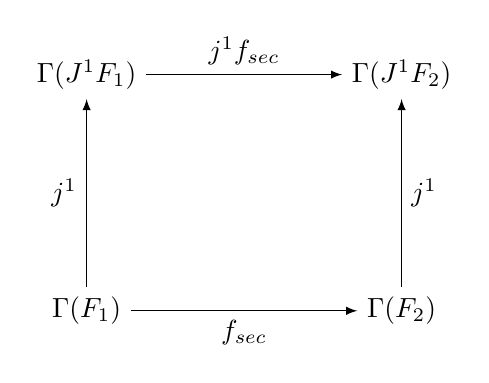
\begin{tikzpicture}
\node (F1) at (0,0) {$\Gamma(F_1)$};
\node (F2) at (4,0) {$\Gamma(F_2)$};
\node (JF1) at (0,3) {$\Gamma(J^1F_1$)};
\node (JF2) at (4,3) {$\Gamma(J^1F_2)$};
\draw [-latex] (F1) -- node[pos=0.5, below] {$f_{sec}$} (F2);
\draw [-latex] (JF1) -- node[pos=0.5, above] {$j^1f_{sec}$} (JF2);
\draw [-latex] (F1) -- node[pos=0.5, left] {$j^1$} (JF1);
\draw [-latex] (F2) -- node[pos=0.5, right] {$j^1$} (JF2);
\end{tikzpicture}
\caption{Commutative Diagram: Prolongation of Bundle Morphisms Applied to Sections.}\label{BundleMorphSec}
\end{figure}

We can prolong bundle morphisms to any higher-order jet bundle by an equivalent definition, i.e., by defining $j^k(f)$ s.t. the diagram in Figure \ref{POrolongK} commutes:
\begin{figure}[hbt!]
\centering
\begin{tikzpicture}
\node (M) at (0,0) {$M$};
\node (N) at (5,0) {$N$};
\node (F1) at (0,3) {$F_1$};
\node (F2) at (5,3) {$F_2$};
\node (JF1) at (0,6) {$J^kF_1$};
\node (JF2) at (5,6) {$J^kF_2$};
\draw [-latex] (M.10) -- node[pos=0.5, above] {$\phi$} (N.170);
\draw [<-] (M.350) -- node[pos=0.5, below] {$\phi^{-1}$} (N.190);
\draw [-latex] (F1) -- node[pos=0.5, above] {$f$} (F2);
\draw [-latex] (F1) -- node[pos=0.5, left] {$\pi_{F_1}$} (M);
\draw [-latex] (F2) -- node[pos=0.5, right] {$\pi_{F_2}$} (N);
\draw [-latex] (JF1) -- node[pos=0.5, left] {$(\pi_1)_{k,0}$} (F1);
\draw [-latex] (JF2) -- node[pos=0.5, right] {$(\pi_2)_{k,0}$} (F2);
\draw [-latex] (JF1) -- node[pos=0.5, above] {$j^k(f)$} (JF2);
\end{tikzpicture}
\caption{Commutative Diagram: Prolongation of Bundle Morphisms to $k$th-order Jet Bundle.} \label{POrolongK}
\end{figure}
One can in particular show that the jet prolongations of bundle morphisms behaves functorial w.r.t. their composition: $j^k(f\circ g) = j^k(f) \circ j^k (g)$. Details regarding the prolongation of bundle morphisms can be found in \cite{saunders_1989}.

Now we are in a position where we can formulate what we mean by requiring the gravitational theory to be invariant under spacetime diffeomorphisms in a precise manner. We start by recalling the definition of an \textit{\textbf{equivariant}} map. Further information regarding this can be found in \cite{doi:10.1142/3867}.
\begin{definition}[equivariance]
Let $M$ and $N$ be some spaces that both carry an action of a group $\mathcal{G}$, $\rho : \mathcal{G} \rightarrow \mathrm{Aut}(M)$ and $\sigma : \mathcal{G} \rightarrow \mathrm{N}$. We call a function $f : M \rightarrow N$ equivariant w.r.t. $\rho$ and $\sigma$ if it holds for all $g \in \mathcal{G}$ that: $f \circ \rho(g) = \sigma(g) \circ f(m)$, i.e. if the diagram displayed in Figure \ref{EquiDia} commutes for all $g \in \mathcal{G}$:
\begin{figure}[hbt!]
\centering
\begin{tikzpicture}
\node (M) at (0,0) {$M$};
\node (N) at (4,0) {$N$};
\node (M2) at (0,3) {$M$};
\node (N2) at (4,3) {$N$};
\draw [-latex] (M) -- node[pos=0.5, below] {$f$} (N);
\draw [-latex] (M2) -- node[pos=0.5, above] {$f$} (N2);
\draw [<-] (M) -- node[pos=0.5, left] {$\rho(g)$} (M2);
\draw [<-] (N) -- node[pos=0.5, right] {$\sigma(g)$} (N2);
\end{tikzpicture}
\caption{Commutative Diagram: Equivariant Map.}\label{EquiDia}
\end{figure}
\end{definition}
Finally, we provide a definition for a \textit{\textbf{diffeomorphism invariant Lagrangian field theory}}.
\begin{definition}
A Lagrangian field theory described by a second-order Lagrangian $\mathcal{L} : J^2F \rightarrow \Lambda^4 M$ is called diffeomorphism invariant if $\mathcal{L}$ is equivariant w.r.t. the action of $\mathrm{Diff}(M)$ that is obtained by prolonging diffeomorphisms to bundle isomorphisms of $J^2F$ and the pullback action of diffeomorphisms on $\Lambda^4M$, i.e., if it holds for all $\phi \in \mathrm{Diff}(M)$ that: 
\begin{align}
     \mathcal{L}\circ j^2(\phi_{\ast}) = \phi_{\ast} \circ \mathcal{L}.
\end{align}
\end{definition}

\textit{\textbf{Infinitesimally}}, on the \textbf{\textit{Lie algebra}} level, diffeomorphisms are described by vector fields $\xi \in \Gamma(M)$ with Lie bracket being provided by the commutator of vector fields. 
As usual, one can derive an action of a Lie algebra from a given action of the corresponding Lie group.
Given a Lie group action of some Lie group $\mathcal{G}$ on some manifold $M$, i.e. $\rho : \mathcal{G} \rightarrow \mathrm{Aut}(M)$, one defines for all $p \in M$ the the orbit map:
\begin{align}
    \begin{aligned}
    \rho_p : \mathcal{G} &\longrightarrow M \\
    g &\longmapsto \rho(g)(p).
    \end{aligned}
\end{align}
This map is differentiable. Its push forward at the identity of $\mathcal{G}$ yields for each element of the Lie algebra of $\mathcal{G}$ a tangent vector at $p$ . Repeating this process for each $p \in M$ one obtains a vector field on $M$. It can then be shown that mapping each $\xi \in \mathrm{Lie}(\mathcal{G})$ to the negative of this vector field defines a morphism of Lie algebras $\mathrm{Lie}(\mathcal{G}) \rightarrow \Gamma(TM)$, i.e. a Lie algebra action of $\mathrm{Lie}(\mathcal{G})$ on $M$. For details see for instance \cite{boothby1989} and \cite{doi:10.1142/3867}.
Hence this procedure allows one to derive a Lie algebra action from a given Lie group action. Recall that we already have deduced how diffeomorphisms act on the field bundle $F$ and also on the jet bundles defined over it. Thus we can now use the construction outlined above to obtain from these actions of diffeomorphisms \textit{\textbf{Lie algebra morphisms}} that describe how infinitesimal diffeomorphisms act on these bundles.
Note that, for the special case of the pullback action of diffeomorphism on tensor bundles $T^m_nM$ over $M$, given a $\xi \in \Gamma(TM)$ the induced action of the corresponding vector field on $T^m_nM$ on sections $G \in \Gamma(T^m_nM)$ is usually called the \textit{\textbf{Lie derivative}} and denoted by $G \mapsto \mathcal{L}_{\xi}G$. 

We start by applying the above construction to the pullback action of diffeomorphisms on the field bundle in coordinates $x^m$ on $M$, adapted coordinates $(x^m, v_A)$ on $F$ and the corresponding induced coordinates on $TM$ and $TF$ respectively, this Lie algebra morphism takes the following form:
\begin{align}\label{LieF}
\begin{aligned}
    \mathcal{f} : \Gamma(TM) &\longrightarrow \Gamma(TF)\\
    \xi &\longmapsto \xi_F \\
    \smallskip
    \xi_F = \xi^m \frac{\partial}{\partial x^m} + \xi^A \frac{\partial}{\partial v_A} &= \xi^m \frac{\partial}{\partial x^m} + C_{An}^{Bm} v_B \partial_m \xi ^n \frac{\partial}{\partial v_A}. 
\end{aligned}
\end{align}
Here the constant tensor $C_{An}^{Bm}$ describes the vertical part of $\xi_F$, i.e. the part of the vector field that lies in the kernel of $(\pi_F)_{\ast}$. We will call $C_{An}^{Bm}$ the \textit{\textbf{vertical coefficient}} of the infinitesimal  diffeomorphism action on $F$. The precise form of the vertical coefficient clearly depends on the specific nature, i.e., rank and symmetries of the tensor fields in consideration.
It can most easily be computed by making use of the standard rules of computing Lie derivatives in coordinates and further using:
\begin{align}
    \mathcal{L}_{\xi} G_A = \partial_m G_A \xi^m + C_{An}^{Bm} G_B \partial_m \xi ^n.
\end{align}
The only feature that all possible vertical coefficients $C_{An}^{Bm}$ have in common, irrespective of the specific field bundle at hand is that they will always be given in a way that ensures that $\mathcal{f}$ defines a Lie algebra morphism, i.e, 
\begin{align}
\mathcal{f}\bigl ( \bigl [\xi, \tilde{\xi} \bigr ]_{\Gamma(TM)}\bigr ) = \bigl [ \mathcal{f}\bigl (\xi\bigr ), \mathcal{f}\bigl (\tilde{\xi}\bigr ) \bigr]_{\Gamma(TF)}
\end{align}
Similarly, we can now compute the Lie algebra action that corresponds to the prolonged actions on $J^1F$ and $J^2F$. By doing this, we obtain \textbf{\textit{prolonged}} vector fields that describe the infinitesimal diffeomorphism action on the jet bundle. In coordinates $(x^m,v_A,v_{Ai})$ on $J^1F$ we obtain:
\begin{align}
    \begin{aligned}
    j^1(\mathcal{f}) : \Gamma(TM) &\longrightarrow \Gamma(TJ^1F)\\
    \xi & \longmapsto \xi_{J^1F}.
    \end{aligned}
\end{align}
Where we can compute the thus prolonged vector field $j^1(\xi)$ to be given by 
\begin{multline}\label{LieJ1}
    \xi_{J^1F} = \xi^m \frac{\partial}{\partial x^m} + C_{An}^{Bm} v_B \partial_m \xi ^n \frac{\partial}{\partial v_A}\\
    + C_{An}^{Bm} \partial_m \xi^n v_{Bi} \frac{\partial}{\partial v_{Ai}} - v_{An} \partial_m \xi ^n \frac{\partial}{\partial v_{Am}} + C_{An}^{Bm} v_B \partial_m \partial_p \xi^n \frac{\partial}{\partial v_{Ap}}.
\end{multline}
In precisely the same way one can now construct prolongations of vector field to higher-order jet bundles as for instance to the second-order jet bundle as it is relevant for our treatment of Lagrangian field theory.
\begin{align}
    \begin{aligned}
    j^2(\mathcal{f}) : \Gamma(TM) &\longrightarrow \Gamma(TJ^2F)\\
    \xi & \longmapsto \xi_{J^2F}.
    \end{aligned}
\end{align}
Performing a similar computation as before in adapted coordinates $(x^m,v_A,v_{Ai}, v_{AI})$ on $J^2F$, we find:
\begin{align}\label{LieJ2}
\begin{aligned}
    \xi_{J^2F} = &\hphantom{-} \xi^m \frac{\partial}{\partial x^m} + C_{An}^{Bm} v_B \partial_m \xi ^n \frac{\partial}{\partial v_A}
    + C_{An}^{Bm} \partial_m \xi^n v_{Bi} \frac{\partial}{\partial v_{Ai}}\\
    &- v_{An} \partial_m \xi ^n \frac{\partial}{\partial v_{Am}} + C_{An}^{Bm} v_B \partial_m \partial_p \xi^n \frac{\partial}{\partial v_{Ap}} 
    + C_{An}^{Bm} v_{BI} \partial_m \xi ^n \frac{\partial}{\partial v_{AI}}\\
    &- 2 v_{BJ} I^J_{an}J^{am}_I \partial_m \xi^n \frac{\partial}{\partial v_{AI}} + 2 C_{An}^{Bm} v_{Ba}J^{ap}_I \partial_m \partial_p \xi^n \frac{\partial}{\partial v_{AI}}\\
    &- v_{An} J^{pm}_I \partial_m \partial_p \xi^n\frac{\partial}{\partial v_{AI}} + C_{An}^{Bm} v_B J^{pq}_I \partial_m \partial_p \partial_q \xi^n \frac{\partial}{\partial v_{AI}}.
\end{aligned}
\end{align}
These two expressions describe the infinitesimal action of a diffeomorphism that is induced by a vector field $\xi$ on the first and second jet bundle over the field bundle, respectively. 
All the involved maps, $j^1(\mathcal{f})$ and $j^2(\mathcal{f})$ or in fact any prolongation to any higher jet bundle $j^q(\mathcal{f})$ define Lie algebra morphisms, and hence one, in particular, finds that they preserve the commutator:
\begin{align}
j^q (\mathcal{f})\bigl (  \bigl [\xi, \tilde{\xi}  \bigr ]_{\Gamma(TM)}\bigr) =  \bigl [ j^q(\mathcal{f})(\xi), j^q(\mathcal{f})(\tilde{\xi}) \bigr ]_{\Gamma(TJ^qF)}
\end{align}
Using the prolongation of vector fields to the jet bundle we can now state one of the main results regarding the implications of the diffeomorphism equivariance of bundle maps on the jet bundle. We present a first-order PDE system that
such an equivariant bundle map necessarily has to solve. 
This, of course, also applies to the special case of the bundle map in consideration being
the Lagrangian of a diffeomorphism invariant field theory. 
\begin{theorem}[equivariance equations]
Let $(F,\pi_f,M)$ be the field bundle and $J^2F$ denote the second-order jet bundle over $F$. Furthermore let $(E, \pi_E, M)$ be a second bundle over $M$ with adapted coordinates $(x^m, u_{\tilde{A}})$ that carries an action of $\mathrm{Diff}(M)$ which is infinitesimally described by a Lie alegbra morphism $\mathcal{e}: \Gamma(TM) \rightarrow \Gamma(TE)$ with coordinate expression $\mathcal{e}(\xi) = \xi^m \frac{\partial}{\partial x^m} + K_{\tilde{A}n}^{\tilde{B}m} u_{\tilde{B}} \partial_m \xi^n \frac{\partial}{\partial u_{\tilde{A}}}$. Assume that we are given a bundle morphism $f : J^2F \rightarrow E$ covering $id_M$ that is equivariant w.r.t. the lifted action of $\mathrm{Diff}(M)$ on $J^2F$ and the action $\mathcal{e}$ on $E$, then in coordinates $f^{\tilde{A}}$ satisfies the following set of linear first-order partial differential equations:
\begin{align}
\begin{aligned}
    0 &= f^{\tilde{C}:m} \\
    0 &= f^{\tilde{C}:A} C_{An}^{Bm} v_B + f^{\tilde{C}:Ap} \bigl[ C_{An}^{Bm} \delta_p^q - \delta_A^B \delta_m^n \bigr] v_{Bq} + f^{\tilde{C}:AI} \bigl[ C_{An}^{Bm} \delta_I^J - 2 \delta_A^B J_I^{pm} I^J_{pn}  \bigr] v_{BJ} - f^{\tilde{A}}K_{\tilde{A}n}^{\tilde{C}m}\\
    0 &= f^{\tilde{C}:A(p\vert}C_{An}^{B \vert m)} v_B + f^{\tilde{C}: AI} \bigl[ C_{An}^{B(m\vert} 2 J_I^{\vert p) q} - \delta^B_A J_I ^{pm} \delta_n^q \bigr] v_{Bq} \\
    0 &= f^{\tilde{C}:AI} C_{An}^{B(m\vert} v_B J_I^{\vert p q )}.
\end{aligned}
\end{align}
\end{theorem}
Here we introduced the notation $h^{:A} := \partial^A h$. The four equations describe a system of first-order partial differential equations (PDEs) for the coordinate representation of $f$. 
\begin{proof}
The statement follows immediately from the definition of equivariance. Evaluating this definition infinitesimally, i.e., on the level of Lie algebra actions for some vector field $\xi$ we obtain an equality with left-hand side being given by the application of the prolonged vector field $\xi_{J^2F}$ and right-hand side given as: $f^{\tilde{A}}K_{\tilde{A}n}^{\tilde{C}m} \partial_m \xi^n$. As this equation has to hold for arbitrary vector fields, $\xi$, we can, in particular, use $\xi$ to isolate contributions from specific derivatives. 
For instance by taking the components of the vector field as $\xi^a = \delta^a_2$ we only get contributions proportional to $\xi^2$. Thus we can conclude that these contributions have to vanish separately. Choosing further $\xi^a = \delta^a_2 x^3$ only terms that either contain $\xi^2$ or $\partial_3 \xi^2$ are non-zero. As priorly we already have deduced that those terms containing $\xi^2$ have to vanish separately we can now follow that also those that are proportional to $\partial_3 \xi ^2$ must vanish independently of the remaining contributions.
Hence we can equate the coefficients of different derivatives of $\xi$ to zero independently, which then yields the desired PDE system and therefore proves the statement.  
\end{proof}
The PDE system deduced from the equivariance of $f$ can, obviously, be projected to a PDE system encoding equivariance for functions on $J^1F$. This is done by discharging all terms that contain derivatives w.r.t. second-order jet coordinates $v_{AI}$. 
Simirlar PDEs can also be obtained for equivariant functions on higher-order jet bundles.
Note that from the last theorem we can conclude in particular that the Lagrangian of diffeomorphisms invariant field theories, in local coordinates given by $\mathcal{L} = L \mathrm{d}^4x$ on $J^2F$ satisfies the following linear first-order PDE system:  
\begin{align}\label{DiffeoEqn}
\begin{aligned}
    0 &= L^{:m} \\
    0 &= L^{:A} C_{An}^{Bm} v_B + L^{:Ap} \bigl[ C_{An}^{Bm} \delta_p^q - \delta_A^B \delta_m^n \bigr] v_{Bq} + L^{:AI} \bigl[ C_{An}^{Bm} \delta_I^J - 2 \delta_A^B J_I^{pm} I^J_{pn}  \bigr] v_{BJ} + L \delta^m_n \\
    0 &= L^{:A(p\vert}C_{An}^{B \vert m)} v_B + L^{: AI} \bigl[ C_{An}^{B(m\vert} 2 J_I^{\vert p) q} - \delta^B_A J_I ^{pm} \delta_n^q \bigr] v_{Bq} \\
    0 &= L^{:AI} C_{An}^{B(m\vert} v_B J_I^{\vert p q )}.
    \end{aligned}
\end{align}
The only ingredient that explicitly depends on the particular nature of the field is the vertical coefficient tensor $C^{Bm}_{An}$.
The remaining objects in (\ref{DiffeoEqn}) take precisely this form no matter what concrete field theory we wish to consider.
Considering field theories on $J^1F$ this was already presented in \cite{Gotay1992StressEnergyMomentumTA}, where the authors used a similar PDE system for the Lagrangian to construct a universal energy-momentum tensor that is conserved for any diffeomorphism invariant field theory.

In the context of Constructive Gravity, it is worth to mention that as we required diffeomorphism invariance of the gravitational theory, any Lagrangian that might describe it necessarily needs to solve the PDE system (\ref{DiffeoEqn}). To put it differently, by finding the general solution to the Lagrangian equivariance PDE for a given gravitational field bundle we would obtain the broadest possible set of candidates for the Lagrangian of this theory of gravity. Without further requirements of the gravitational theory finding Lagrangians that describe the diffeomorphism invariant gravitational dynamics of a given gravitational field, therefore, boils down to solving the above PDE system (\ref{DiffeoEqn}). 

From the diffeomorphism equivariance equations, we easily see that in order to simplify the task of solving the system, we might proceed as follows:
We first solve the corresponding \textit{\textbf{invariance equation}}, the system (\ref{DiffeoEqn}) with the second equation being replaced by the corresponding homogeneous equation
\begin{align}
    0 &= L_{scal}^{:A} C_{An}^{Bm} v_B + L_{scal}^{:Ap} \bigl[ C_{An}^{Bm} \delta_p^q - \delta_A^B \delta_m^n \bigr] v_{Bq} + L_{scal}^{:AI} \bigl[ C_{An}^{Bm} \delta_I^J - 2 \delta_A^B J_I^{pm} I^J_{pn}  \bigr] v_{BJ}.
\end{align}
A solution to this system describes a map $L_{scal}: J^2F \rightarrow \mathbb{R}$ that is invariant under diffeomorphisms, i.e. for all $\phi \in \mathrm{Diff}(M)$ it holds that:
\begin{align}
    L_{scal} \circ j^2(\phi) = L_{scal}.
\end{align}
Once we obtain the general solution to these diffeomorphism invariance equations, $L_{scal}$ multiplying by any particular solution of (\ref{DiffeoEqn}) yields a solution of the diffeomorphism equivariance equations. We might, for instance, take this particular solution to only depend on the coordinates of $F$ and not on the derivative coordinates. Such solutions can typically be found more easily as then all terms in (\ref{DiffeoEqn}) that contain derivatives w.r.t. the derivative coordinates on $J^2F$ drop out. Conversely given any two solutions to the equivariance equations taking their quotient yields a solution to the invariance equations. These arguments show that there really is a one to one correspondence between solutions of the equivariance and invariance equations. Whether or not solving the invariance equation gives advantages over solving the PDE (\ref{DiffeoEqn}) can only be decided with concrete examples at hand. Details regarding these considerations can be found in Theorem \ref{GeneralSol} and the corresponding proof. 

Note that the first equation in the PDE system (\ref{DiffeoEqn}) simply requires the Lagrangian to be independent of the coordinates of the spacetime manifold. This is, of course, a requirement posed on the Lagrangian as a bundle map on $J^2F$, not on the corresponding composition with a given section of $J^2F$ as all such compositions are necessary $x^m$-dependent. The first equation can hence be trivially solved, and we might use its implications in the following. For instance, we can now write $L(v_A.v_{Ai},v_{AI})$ for the coordinate expression of the Lagrangian, discharging the explicit $x^m$-dependency.

Before proceeding with the next section, we quickly deduce the implications for the EOM that are generated by diffeomorphism invariant Lagrangians. The EOM of a given Lagrangian $\mathcal{L}$ can be obtained by taking its variational derivative, in coordinates $E^A := \frac{\delta \mathcal{L}}{\delta v_A}$, composing it with the prolongation of a section of the field bundle and then equating to zero. In the following, we will also refer to $E^A$ as equations of motion. If the Lagrangian is given as a function on the second jet bundle, then the EOM are generally functions on the fourth jet bundle $J^4F$. As mentioned before we are however particularly interested in the case where the Lagrangian is degenerated in the sense that also the EOM are functions on $J^2F$, and hence a meaningful Hamiltonian formulation exists.
\begin{theorem}[diffeomorphism equivariant EOM]
Given a Lagrangian on $J^2F$ that describes a diffeomorphism invariant field theory with second-order EOM, in the usual coordinates: $E^A := \frac{\delta \mathcal{L}}{\delta v_A}$, then the equations of motion satisfy the following linear first-order PDE system:
\begin{align}\label{EOM}
    \begin{aligned}
    0 &= E^{C:m} \\
    0 &= E^{C:A} C_{An}^{Bm} v_B + E^{C:Ap} \bigl[ C_{An}^{Bm} \delta_p^q - \delta_A^B \delta_m^n \bigr] v_{Bq} + E^{C:AI} \bigl[ C_{An}^{Bm} \delta_I^J - 2 \delta_A^B J_I^{pm} I^J_{pn}  \bigr] v_{BJ}\\
    &+ E^C \delta^m_n + E^A C_{An}^{Cm}  \\
    0 &= E^{C:A(p\vert}C_{An}^{B \vert m)} v_B + E^{C: AI} \bigl[ C_{An}^{B(m\vert} 2 J_I^{\vert p) q} - \delta^B_A J_I ^{pm} \delta_n^q \bigr] v_{Bq} \\
    0 &= E^{C:AI} C_{An}^{B(m\vert} v_B J_I^{\vert p q )}.
    \end{aligned}
\end{align}
\end{theorem}
\begin{proof}
Again we start with Lie algebra version of the equivariance condition for $\mathcal{L}$ and an arbitrary vector field $\xi$. This time the statement can be proven by first computing the variational derivative, i.e., acting with $\frac{\delta}{\delta v_A}$ on the whole equation and then equating the components in front of different derivatives of $\xi$ individually to zero. 
\end{proof}

Similar equations were obtained in the context of variational calculus and gauge symmetries of a given Lagrangian in \cite{article}. In the context of GR, although not in the form of a PDE system, Lovelock used comparable implications deduced from the required diffeomorphism invariance to prove that the Einstein-Hilbert-Lagrangian is unique in the sense that it is the only Lagrangian producing second-derivative-order EOM that solves these implications \cite{Lovelock1969}, \cite{doi:10.1063/1.1666069} and \cite{doi:10.1063/1.1665613}. 

If we loosen our requirements of the gravitational theory to the point where we are only interested in the EOM and not the Lagrangian, we could also work with the PDE system (\ref{EOM}). By solving this system, we obviously directly obtain EOM. Such an approach is described in \cite{TobiR}.

Summing up we have derived linear first-order PDE systems for the Lagrangian or the equations of motion respectively that encode the required diffeomorphism invariance of a given field theory. Any theory that is invariant under spacetime diffeomorphisms has to solve the two PDEs. Conversely, we might construct diffeomorphism invariant theories as solutions to either the system (\ref{DiffeoEqn}) on the level of the Lagrangian or the system (\ref{EOM}) on the level of the EOM. This is a massive improvement as now the notoriously difficult requirement of diffeomorphism invariance that we have posed on the gravitational theory that we wish to construct is translated into the rather simple quest of solving a linear first-order PDE system.  



\section{Canonical Kinematics and Hypersurface Deformations}
In the following two sections we are going to investigate the implication of the required diffeomorphism invariance for the \textit{\textbf{canonical formulation}} of a given field theory. For that purpose we mainly concern field theories that are described by a \textit{\textbf{first-order}} Lagrangian, i.e., a function on $J^1F$. Working on $J^2F$ as before we would necessarily have to consider the case where the Lagrangian is degenerate such that the EOM are nevertheless of second-order and the Hamiltonian formulation is free of Ostrogratsky instabilities. The degeneracy of the Lagrangian would then, however, impede the canonical formulation of the theory\footnote{We remark that, although posing further technical difficulties, we expect a generalization of the following derivations to the case of degenerate Lagrangians on $J^2F$ to be straight forward.}.

The main idea that is used when transferring from a given Lagrangian field theory to the associated Hamiltonian formulation is that of decomposing the spacetime manifold $M$ into a disjoint set of 3-dimensional manifolds that are smoothly parametrized by a time parameter. As a consequence, one can then accordingly decompose any structure that is prescribed on $M$. In order to achieve this we follow \cite{2004math.ph..11032G} and introduce the notion of a \textit{\textbf{slicing}}, sometimes also called a \textit{\textbf{3+1-split}}, of the spacetime manifold $M$.
\begin{definition}[slicing]
A slicing of the spacetime manifold $M$ is a diffeomorphism 
\begin{align}
\phi : \Sigma \times \mathbb{R} \longrightarrow M.
\end{align}
\end{definition}
By this definition for each $\lambda \in \mathbb{R}$ we obtain an embedding $\phi_{\lambda}$ of the 3-dimensional manifold $\Sigma$:
\begin{align}
\begin{aligned}
\phi_{\lambda}: \Sigma &\longrightarrow M \\
s &\longmapsto \phi_{\lambda}(s) := \phi(s,\lambda).
\end{aligned}
\end{align}
We define the images of this one-parameter family of embeddings as $\Sigma_{\lambda} := \phi_{\lambda}(\Sigma)$. Hence we can think of the embedded 3-dimensional manifolds $\Sigma_{\lambda}$ as modelling space at given parameter time $\lambda$.
Note that it is a priori not clear whether or not such a slicing exists for a given spacetime $M$. For the situation in Constructive Gravity, or physics in general, there are, however, certain results that guaranty its existence. If we require that the spacetime manifold can additionally be endowed with a predictive matter field theory --- predictive in the sense that the corresponding matter field EOM are of hyperbolic type\footnote{We will provide a rigorous version of this statement in the second chapter. } --- then one can show that there necessarily exists a slicing of spacetime with the embedded spaces $\Sigma_{\lambda}$ being initial data hypersurfaces for the hyperbolic EOM. This is undoubtedly a requirement that is necessary if we want to be able to make physical predictions. For further details see for instance \cite{2003CMaPh.243..461B} for the situation in GR, and also \cite{1996gere.conf...19G} for a more general context. 

\begin{figure}[hbt!]
\centering
\begin{tikzpicture}
\node (S) at (0,0) {$\Sigma \times \mathbb{R}$};
\node (M) at (4,0) {$M$};
\node (R) at (0,-4) {$\mathbb{R}$};
\draw [<-] (S) -- node[pos=0.5, above] {$\phi^{-1}$} (M);
\draw [-latex] (S) -- node[pos=0.5, left] {$\pi_{\mathbb{R}}$} (R);
\draw [-latex] (M) -- node[pos=0.5, right] {$t$} (R);
\end{tikzpicture} 
\caption{Commutative Diagram: Slicing induced Time Function.}\label{DiagrTime}
\end{figure}

In addition to the smoothly parameterized family of embeddings $\phi_{\lambda}$ a slicing on $M$ immediately induces a \textit{\textbf{time vector field}} and a \textit{\textbf{time differential}} one form on $M$. The one form can be obtained as differential $\mathrm{d}t$ of the function $t:=\pi_{\mathbb{R}} \circ \phi^{-1}$, where $\pi_{\mathbb{R}}$ denotes the canonical project of $\Sigma \times \mathbb{R}$ onto the second factor. The situation is displayed in Figure \ref{DiagrTime}.
The time vector field can be constructed by first defining for all $s \in \Sigma$ the following map: 
\begin{align}
\begin{aligned}
    \phi_s : \mathbb{R} &\longrightarrow M \\
    \lambda &\longmapsto \phi(s,\lambda).
\end{aligned}
\end{align}
These maps define curves on $M$. They track the path of specific spatial point $s \in \Sigma$ through spacetime, defined by the family of embeddings. The situation can be seen in Figure \ref{Slicing}.

\begin{figure}[hbt!]
\centering
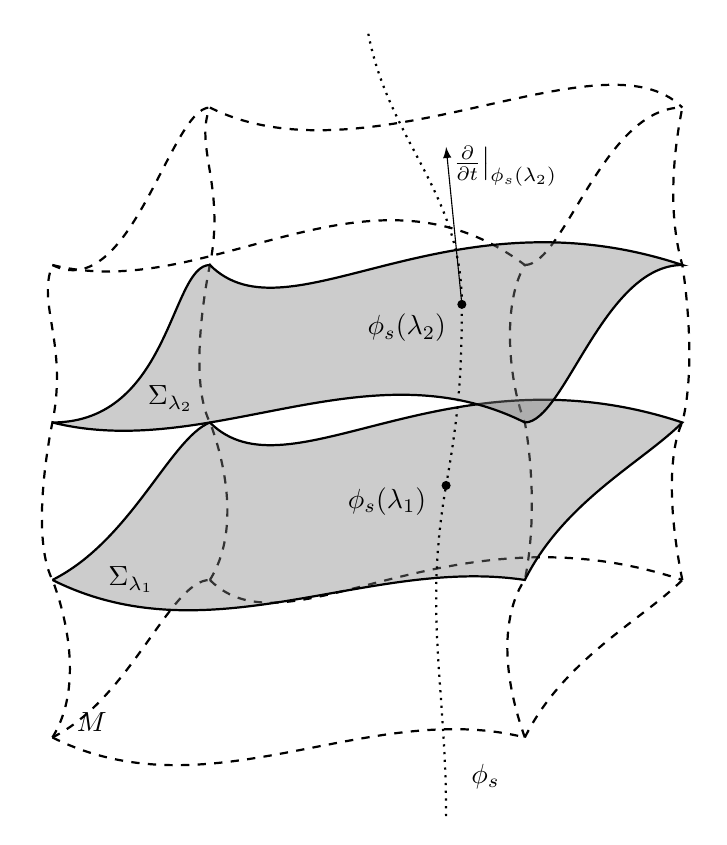
\begin{tikzpicture}
\draw[thick, dashed] (0,0) .. controls (2,-1) and (4,0.5)  .. (6,0);
\draw[thick, dashed] (0,0) 
.. controls (0.5,0.8) and (0,2) ..
(0,2) .. controls (-0.3,2.6) and (0,4) ..
(0,4) .. controls (0.2,5) and (-0.2,5.5) .. (0,6);
\draw[thick, dashed] (6,0)  
.. controls (5.5,1.4) and (6,2) ..
(6,2) .. controls (6.2,3) and (6,4) ..
(6,4) .. controls (5.8,4.5) and (5.7,5.5) .. (6,6);
\draw[thick, dashed] (0,6) .. controls (2,5.5) and (4,7.5) .. (6,6);
\draw[thick, dashed] (0,0) .. controls (1,0.5) and (1.5,2) .. (2,2);
\draw[thick, dashed] (6,0)  .. controls (6.5,1) and (7.5,1.5) .. (8,2);
\draw[thick, dashed] (6,6) .. controls (6.5,6) and (7,8) ..  (8,8);
\draw[thick, dashed] (0,6) .. controls (1,5.5) and (1.5,8) .. (2,8);
\draw[thick, dashed] (2,2) .. controls (3,1) and (5,3) .. (8,2);
\draw[thick, dashed] (2,2) 
.. controls (2.5,2.8) and (2,4) ..
(2,4) .. controls (1.7,4.6) and (2,6) ..
(2,6) .. controls (2.2,7) and (1.8,7.5) .. (2,8);
\draw[thick, dashed] (8,2)   
.. controls (7.7,3.5) and (8,4) ..
(8,4) .. controls (8.2,4.8) and (8,6) ..
(8,6) .. controls (7.8,6.7) and (7.9,7.5) ..  (8,8);
\draw[thick, dashed] (2,8)  .. controls (4,7) and (7,9) .. (8,8);

\draw[thick, draw = black, fill = gray, fill opacity = 0.4] (0,2) .. controls (2,1) and (4,2.3) ..
(6,2)  .. controls (6.5,3) and (7.5,3.5)..
(8,4) .. controls (5,5) and (3,3) ..
(2,4) .. controls (1.5,3.8) and (1,2.5)  .. (0,2); 

\draw[thick, draw = black, fill = gray, fill opacity = 0.4] (0,4) .. controls (2,3.5) and (4,5) ..
(6,4)  .. controls (6.5,4) and (7,6)..
(8,6) .. controls (5,7) and (3,5) ..
(2,6) .. controls (1.5,6) and (1.5,4)  .. (0,4); 

\node (M) at (0.5,0.2) {$\boldsymbol{M}$};
\node (S1) at (1,2) {$\boldsymbol{\Sigma_{\lambda_1}}$};
\node (S2) at (1.5,4.3) {$\boldsymbol{\Sigma_{\lambda_2}}$};

\draw[fill] (5,3.2) circle [radius=0.05];
\node (P1) at (4.25,3)
{$\phi_s(\lambda_1)$};
\draw[fill] (5.2,5.5) circle [radius=0.05];
\node (P1) at (4.5,5.2)
{$\phi_s(\lambda_2)$};

\draw[thick, dotted] (5,-1) to [out = 90, in = 260] (5,3.2);
\draw[thick, dotted] (5,3.2) to [out = 80, in = 270] (5.2,5.5);
\draw[thick, dotted] (5.2,5.5) to [out = 90, in = 280] (4,9);
\node at (5.5,-0.5)
{$\phi_s$};
\draw[-latex] (5.2,5.5) to (5,7.5); 
\node at (5.75,7.25) {$\frac{\partial}{\partial t}\big \vert _{\phi_s(\lambda_2)}$};
\end{tikzpicture} 
\caption{Slicing of Spacetime into 3-dimensional Slices.}\label{Slicing}
\end{figure}
Therefore each such curve provides us with tangential vectors along it. Using this we can define a vector field on $M$ by defining the value at $p \in M$ to be given by the tangential vector of the specific such curve that is passing through $p$:
\begin{align}
\frac{\partial}{\partial t}\bigg \vert_p = \phi^{\prime}_{\pi_{\Sigma}\circ \phi^{-1}(p)} \left (\pi_{\mathbb{R}}\circ \phi^{-1}(p)\right ).
\end{align}
One readily finds that $\frac{\partial}{\partial t}$ and $\mathrm{d}t$ are dual objects, i.e. $\mathrm{d}t(\frac{\partial}{\partial t}) = 1$ and hence the notation. In the following we call $t$ time function, $\mathrm{d}t$ time differential and $\frac{\partial}{\partial t}$ time vector field.


Given the fact that $\mathrm{d}t$ and $\frac{\partial}{\partial t}$ were obtained from the given slicing this immediately raises the question of how the time differential, time vector field, and all further objects that will subsequently be defined in terms of these, change under a change of slicing. If $\phi : \Sigma \times \mathbb{R} \rightarrow M $ and $\psi : \Sigma \times \mathbb{R} \rightarrow M$ are two slicings then we obtain a diffeomorphism on $M$ by taking $\psi \circ \phi^{-1}$. Conversely given a slicing $\phi$ any diffeomorphism $\rho \in \mathrm{Diff}(M)$ defines a second slicing by $\rho \circ \phi $. Hence changing the slicing is in one to one correspondence with diffeomorphisms on $M$. 

In addition to the time differential and time vector field on $M$ a slicing also induces a \textbf{\textit{direct sum split}} of the tangent bundle over $M$. Given a slicing $\phi : \Sigma \times \mathbb{R} \rightarrow M$ we can compute its push forward to obtain a vector bundle isomorphism
\begin{align}
\phi_{\ast}: T(\Sigma \times \mathbb{R}) \longrightarrow TM.
\end{align}
Any tangent space over a product of manifolds can be decomposed into a direct sum of the tangent spaces of the individual factors. More precisely one can show that $T(\Sigma \times \mathbb{R}) \cong \pi_{\Sigma}^{\ast}T\Sigma \oplus \pi_{\mathbb{R}}^{\ast} T\mathbb{R}$. And hence in total we have: $TM \cong \pi_{\Sigma}^{\ast}T\Sigma \oplus \pi_{\mathbb{R}}^{\ast} T\mathbb{R}$.
Here $\pi_{\Sigma}^{\ast}T\Sigma$ and $\pi_{\mathbb{R}}^{\ast}T\mathbb{R}$ denote the pullbacks\footnote{Given a bundle $(F,\pi_F,M)$ and a map $h: N \rightarrow M$, the pullback of the bundle $F$ along $h$ is the bundle over $N$ with total space $h^{\ast}F := \{ (n,f) \in N \times F \ \vert \  h(n) = \pi_F(f)\}$, and bundle projection $\pi_{h^{\ast}F}(n,f) = n$ (see \cite{doi:10.1142/3867}). Note that this construction makes the map $\tilde{h}: f^{\ast}F \rightarrow F$ defined by $\tilde{h}(n,f) = f$ a bundle morphism covering $h$, i.e the following diagram commutes. 
\begin{center}
\begin{tikzpicture}
\node (M) at (0,0) {$N$};
\node (N) at (4,0) {$M$};
\node (M2) at (0,2) {$f^{\ast}F$};
\node (N2) at (4,2) {$F$};
\draw [-latex] (M) -- node[pos=0.5, below] {$h$} (N);
\draw [-latex] (M2) -- node[pos=0.5, above] {$\tilde{h}$} (N2);
\draw [<-] (M) -- node[pos=0.5, left] {$\pi_{h^{\ast}F}$} (M2);
\draw [<-] (N) -- node[pos=0.5, right] {$\pi_F$} (N2);
\end{tikzpicture}
\end{center}} of the bundles $T\Sigma$ and $T\mathbb{R}$ over $\Sigma$ and $\mathbb{R}$ to the common base space $\Sigma \times \mathbb{R}$ by making use of the two canonical projections.
Moreover, given two vector bundles $(F,\pi_F,M)$ and $(E,\pi_E,M)$ over the same base space $M$, $F\oplus E$ denotes their direct sum or Whitney sum (for details see the first chapter of \cite{nla.cat-vn705150}). The Whitney sum of two vector bundles is the new vector bundle with fiber at $p \in M$ given by the direct sum of vector spaces $\pi_F^{-1}(p) \oplus \pi_E^{-1}(p)$. 
Note that the Whitney sum can only be constructed for two vector bundles with common base space.
Using the fact that all isomorphisms in the above construction are isomorphisms of vector bundles and thus preserve the Whitney sum decomposition we find that also the spacetime tangent bundle then necessarily decomposes into a Whitney sum. In the following we write
\begin{align}
    TM = \mathcal{T}\Sigma \oplus \mathcal{V}\Sigma
\end{align} 
for this direct sum decomposition of the tangent bundle and call the summands \textit{\textbf{tangential}} and \textit{\textbf{vertical subbundle}} respectively.  
It is important to note that up to technicalities such as the isomorphism $T(\Sigma \times \mathbb{R}) \cong \pi_{\Sigma}^{\ast}T\Sigma \oplus \pi_{\mathbb{R}}^{\ast} T\mathbb{R}$ and also pulling back the bundles along the canonical projections, the tangential and vertical sub bundle of $TM$ are essentially given by the images of $T\Sigma$ and $T\mathbb{R}$ under the pushforward of the slicing $\phi_{\ast}$. 

We can now use this direct sum decomposition of the tangent bundle $TM$ to further decompose structure that is prescibed on it.
In particular vector fields on $M$ can uniquely be \textit{\textbf{decomposed}} w.r.t. this split. Given a vector field $\xi \in \Gamma(TM)$ we write $\xi = \xi_{\parallel} + \xi_{\perp} $ for this decomposition, with $\xi_{\parallel} \in \Gamma(\mathcal{T}\Sigma)$ and $\xi_{\perp} \in \Gamma(\mathcal{V}\Sigma)$ called tangential and vertical part of $\xi$. The situation is drawn in Figue \ref{DecompPic}.

\begin{figure}[hbt!]
\centering
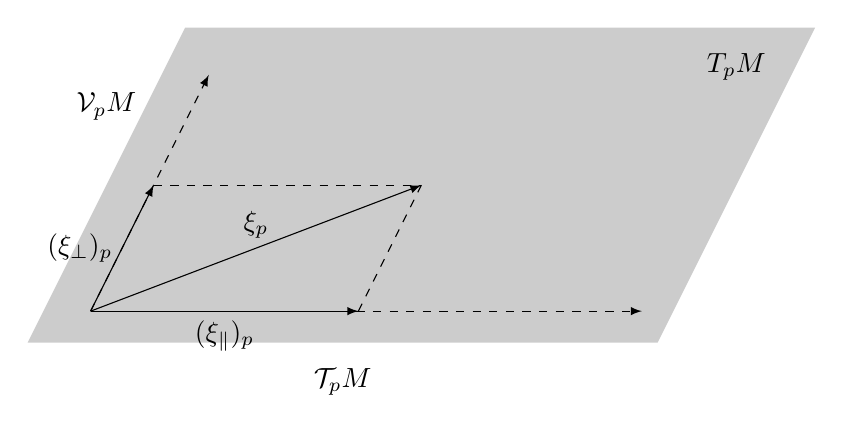
\begin{tikzpicture}
\path[fill = gray, opacity = 0.4] (0,0) -- (8,0) -- (10,4) -- (2,4);
\draw[-latex, dashed] (0.8,0.4) to (2.3,3.4);
\node at (1,3) {$\boldsymbol{\mathcal{V}_pM}$};
\node at (9,3.5) {$\boldsymbol{T_pM}$};
\draw[-latex, dashed] (0.8,0.4) to (7.8,0.4);
\node at (4,-0.5) {$\boldsymbol{\mathcal{T}_pM}$};
\draw[-latex] (0.8,0.4) --  node[pos=0.5, above] {$\boldsymbol{\xi_p}$} (5,2) ;
\draw[-latex] (0.8,0.4) --  node[pos=0.5, left] {$\boldsymbol{(\xi_{\perp})_p}$} (1.6,2) ;
\draw[dashed] (1.6,2) to (5,2);
\draw[-latex] (0.8,0.4) -- node[pos=0.5, below] {$\boldsymbol{(\xi_{\parallel})_p}$} (4.2,0.4);
\draw[dashed] (4.2,0.4) -- (5,2);
\end{tikzpicture}
\caption{Direct Sum Decompostion of Vectors.}\label{DecompPic}
\end{figure}

The vectors in $\mathcal{T}\Sigma$ satisfy: $\mathrm{d}t(\xi_{\parallel})=0$, the vectors in $\mathcal{V}\Sigma$ are parallel to $\frac{\partial}{\partial t}$  . Note that the direct sum split of $TM$ naturally induces a direct some split of the Lie algebra actions on $F$ and $J^1F$ (and also $J^2F$ if we would work on the second-order jet bundle) as the previously constructed Lie algebra morphisms (\ref{LieF}) and (\ref{LieJ1}) are in particular linear maps on the fibers of $TM$ and hence respect the direct sum structure.

We call a coordinate system $(x^m)$ on $M$ \textit{\textbf{adapted}} to the slicing $\phi$ if there exists an adapted coordinate system $(y^{\alpha},z)$ on $\Sigma \times \mathbb{R}$ s.t. $x^0 = z \circ \phi^{-1}$ and $x^{\alpha} = y^{\alpha} \circ \phi^{-1}$. Therefore in adapted coordinates the embedded hypersurfaces are characterized by $x^0 = const$ and the chart induced vector fields satisfy $\frac{\partial}{\partial t} = \lambda \cdot \frac{\partial}{\partial x^0}$ for some $\lambda$ that only depends on $x^0$. We further have $\mathrm{d}t\left(\frac{\partial}{\partial x^{\alpha}}\right) = 0$.
Note that in adapted coordinates we thus find in particular that the induced spatial coordinate fields $\frac{\partial}{\partial x^{\alpha}}$ are sections of the tangential subbundle $\mathcal{T}\Sigma$ whereas $\frac{\partial}{\partial x^0}$ defines a section of the vertical subbundle $\mathcal{V}\Sigma$. Hence in such coordinates, we can express the decomposition of vector fields as 
\begin{align}
    \xi = \xi_{\perp} + \xi_{\parallel} = N  \frac{\partial }{\partial t} + N^{\alpha} \frac{\partial}{\partial x^{\alpha}} = N \cdot \lambda \frac{\partial}{\partial x^0} + N^{\alpha} \frac{\partial}{\partial x^{\alpha}},
\end{align}

In the following, we work mainly over one embedded hypersurface. Given a slicing $\phi$ take some $t_0 \in \mathbb{R}$ and consider the corresponding embedded hypersurface $\Sigma_{t_0}$ with embedding $\phi_{t_0}$. To this end we restrict all functions, fields, etc. on $M$ to $\Sigma_{t_0}$. These restrictions are in the following called \textbf{\textit{hypersurface quantities}}. To keep the notation concise, we might not explicitly denote the restriction every time. 
Furthermore, we find that the restriction of the direct sum split of the tangent bundle to $\Sigma_{t_0}$\footnote{It is important to observe the difference between the restricted tangent bundle $TM\vert_{\Sigma_{t_0}}$ and the tangent bundle of the embedded hypersurface $T\Sigma_{t_0}$. While the former contains a 4-dimensional vector space at each hypersurface point the latter only has 3-dimensional fibers. The difference lies precisely in the vertical bundle over the hypersuface $\mathcal{V}\Sigma_{t_0}$.} is given by $TM \vert _{\Sigma_{t_0}} = T\Sigma _{t_0} \oplus \mathcal{V}\Sigma _{t_0}$. Note that the restriction of the tangential bundle $\mathcal{T}\Sigma_{t_0}$ is precisely given by the tangent bundle over the embedded hypersurface $T\Sigma_{t_0}$.

We are then in particular interested in the question of how hypersurface quantities change under a change of slicing $\phi$ and hence an induced change of the embedding $\phi_{t_0}$. By previous arguments changing the slicing corresponds to the action of a diffeomorphism. Infinitesimally this is described by the Lie algebra action of a vector field $\xi$. Note that whether we can take the standard action of diffeomorphism and vector fields on $M$ or have to take the previously computed lifted actions (\ref{LieF}) on $F$, (\ref{LieJ1}) on $J^1F$, etc. depends on the kind of the objects that we act on.  Given $\xi$, we decompose it into its tangential and vertical part $\xi_{\parallel}$ and $\xi_{\perp}$ to obtain derivative operators that describe the infinitesimal tangential and vertical change of hypersurface quantities.  In adapted coordinates, we obtain such tangential and vertical vector fields by specifying component functions
 $N^a : M \rightarrow \mathbb{R}$ and $N^a : M \rightarrow \mathbb{R}$. We define: 
\begin{align}
    \begin{aligned}
    \mathcal{D}(N^{\alpha}) &:= N^{\alpha} \frac{\partial}{\partial x^{\alpha}} \\
    \mathcal{H}(N) &:= N \frac{\partial}{\partial t} = N \cdot \lambda \frac{\partial}{\partial x^0}.
    \end{aligned}
\end{align} 
Note that we can interpret $\mathcal{D}(N^\alpha)$ and $\mathcal{H}(N)$ as \textit{\textbf{tangential}} and \textit{\textbf{vertical deformation operators}} that when acting on functions compute their infinitesimal change under a tangential respectively vertical deformation by an amount specified by the component functions $N^{\alpha}$ and $N$.
We are now going to compute the commutator algebra that such tangential and vertical vector fields satisfy. Doing this we obtain:
\begin{align}
    \begin{aligned}
    \left [ \mathcal{D}(N^{\alpha}), \mathcal{D}(M^{\alpha}) \right] &= \mathcal{D}(N^\alpha \partial_{\alpha}M^{\beta} - M^{\alpha} \partial_{\alpha} N^{\beta}) \\
    \left[ \mathcal{D}(N^{\alpha}), \mathcal{H}(M) \right] &= \mathcal{H}(N^{\alpha} \partial_{\alpha} M) - \mathcal{D}(M \lambda \partial_0 N^{\alpha})\\
    \left[ \mathcal{H}(N), \mathcal{H}(M) \right ] &= \mathcal{H}(N \lambda \partial_0 M - M \lambda \partial_0N)
    \end{aligned}
\end{align}
Moreover, we want to describe the change in tangential and vertical direction that is computed by the operators $\mathcal{D}(N^{\alpha})$ and $\mathcal{H}(N)$ intrinsically, in terms of quantities that only depend on the coordinates of $\Sigma_{t_0}$.
Hence we restrict the involved component functions $N^{\alpha}$ and $N$ and the deformation operators defined in terms of them such that they locally only depend on the coordinates $x^{\mu}$ and not on $x^0$.
\begin{comment}
The corresponding tangential and vertical vector fields are given by $\mathcal{D}(N^{\alpha})$ and $\mathcal{H}(N)$ can then be interpreted as tangential and vertical deformation operators defined on $\Sigma_{t_0}$. Acting on hypersurface quantities, they compute the infinitesimal change in tangential and vertical direction. Note that the action of vector fields on hypersurface quantities describes their infinitesimal change under diffeomorphisms. Hence by the arguments provided before the action of vector fields on hypersurface quantities describes their infinitesimal change under a change of slicing. The deformation operators $\mathcal{D}(N^{\alpha})$ and $\mathcal{H}(N)$ defined on $\Sigma_{t_0}$ encode contributions to this change in tangential and vertical direction.
\end{comment}
As a consequence contributions from $\partial_0$ derivatives of $N^{\alpha}$ and $N$ now drop out.
We thus obtain the following commutator algebra: 
\begin{align}\label{Alg}
    \begin{aligned}
    \left[ \mathcal{D}(N^{\alpha}), \mathcal{D}(M^{\alpha}) \right] &= \mathcal{D}(\mathcal{L}_{\vec{N}}M^{\beta}) \\
    \left[ \mathcal{D}(N^{\alpha}), \mathcal{H}(M) \right] &= \mathcal{H}(\mathcal{L}_{\vec{N}}M)\\
    \left[ \mathcal{H}(N), \mathcal{H}(M) \right] &= 0,
    \end{aligned}
\end{align}
where we denoted $\mathcal{L}_{\Vec{N}}M^{\beta} = N^\alpha \partial_{\alpha}M^{\beta} - M^{\alpha} \partial_{\alpha} N^{\beta}$ and $\mathcal{L}_{\Vec{N}}M = N^{\alpha} \partial_{\alpha} M$ as Lie derivative along the tangential hypersurface vector field $\vec{N} = N^{\alpha} \frac{\partial}{\partial x^{\alpha}}$ to display the commutator algebra in concise form.
We observe that the commutator of two tangential vector fields again yields a tangential vector field. The tangential vector fields hence constitute a Lie subalgebra. 
The commutator of a tangential and a vertical vector field yields a vertical vector field.
Finally, any two vertical vector fields commute. This commutator algebra encodes the change of hypersurface quantities on $\Sigma_{t_0}$ under a change of the slicing of spacetime. It is therefore often called the \textit{\textbf{hypersurface deformation algebra}}.

\begin{remark}
Note that in traditional terms the hypersurface deformation algebra is mostly obtained by computing commutators of vector fields on the infinite-dimensional manifold of embeddings of a given $\Sigma$ in $M$ (see \cite{HOJMAN197688} and \cite{doi:10.1063/1.522976}). We deliberately decided for an alternative approach here, as already in the formulation of Lagrangian field theory we saw how working with rigorously defined objects constructed over the spacetime manifold instead of a heuristic treatment involving infinite-dimensional function spaces led to a much clearer description that essentially involved the same information. In other words, if working on infinite-dimensional spaces can be avoided, we simply avoid it. We will reencounter this guideline later on when we construct Poisson brackets to incorporate dynamics in terms of the Hamiltonian formulation of field theory.
\end{remark}

One often meets the situation where the direct sum split of the tangent bundle is not obtained from the time vector field $\frac{\partial}{\partial t}$ that is induced by the given slicing, but by means of some physically motivated notion that at each point of the embedded hypersurface $\Sigma_{t_0}$ distinguishes a vertical vector as "time" direction. For instance, this can be achieved by making use of a given \textit{\textbf{observer definition}} for the field theory at hand. For the embedded hypersurface $\Sigma_{t_0}$ one constructs the direct sum split by defining the vertical subbundle as span of the "time" vector field seen as time direction by observers that travel through $p \in \Sigma_{t_0}$ and have a spatial frame lying in the tangent plane $T_p\Sigma_{t_0}$.

Taking the canonical formulation of General Relativity\footnote{For further information regarding some of the provided examples from General Relativity we kindly refer to the standard text books as for instance \cite{Misner1973}. For observer definitions in more general spacetime geometries see \cite{2011PhRvD..83d4047R}.} as an example, given $\Sigma_{t_0}$ and frame fields $e_{\alpha}$ that locally at each point $p \in \Sigma_{t_0}$ in consideration form a basis of $T_p\Sigma_{t_0}$ and satisfy $g(e_{\alpha},e_{\beta}) = \eta_{\alpha \beta}$, to complete the three frame fields to a viable observer frame\footnote{Recall that an observer in GR is defined as a curve $\gamma : \mathbb{R} \rightarrow M$ together with curves $e_{\alpha} : \mathbb{R} \rightarrow TM$, s.t. $ e_a(\lambda) :=(\dot{\gamma}(\lambda),e_{\alpha}(\lambda))$ forms a basis of $T_{\gamma(\lambda)}M$ and $g(e_a(\lambda),e_b(\lambda)) = \eta_{ab}$, , for each $\lambda$.} one needs to choose $e_0$ s.t. 

\begin{align}
    g(e_0,e_0) = 1 \ \text{and} \ g(e_0,e_{\alpha}) = 0.
\end{align}
These two conditions are then often referred to as frame conditions. One can then split the tangent space $T_pM$ at each $p \in \Sigma_{t_0}$ into the vertical part spanned by $e_0(p)$,  $\mathcal{V}_p\Sigma_{t_0} = \langle  e_0(p) \rangle$ and tangential part $T_p\Sigma_{t_0}$ . In particular, one sees that now by the two frame conditions, the vertical time direction and thereby the vertical subbundle and the split itself depend on the metric. Along the same lines given any other field theory with a notion for an observer, one can then use the observer definition to construct the vertical subbundle of $TM$ in a similar fashion. 

One way of defining observers from any given matter field theory that uses the given gravitational field as geometric background can be found in \cite{2018PhRvD..97h4036D} and \cite{2011PhRvD..83d4047R} and also \cite{Rivera}. There the authors construct an observer notion that suits a general gravitational field theory from the \textbf{\textit{Principal Polynomial}}\footnote{Loosely speaking the Principal Polynomial encodes the causal structure of the EOM. In the following chapter, we will encounter this object in more detail.} $\mathcal{P}_{mat}(v_A)$ of the given matter EOM. Note that the Principal Polynomial, in particular, is a function on the field bundle, i.e., is field dependent. The vertical vector field is then obtained in similar fashion compared with the standard GR case. The Principal Polynomial allows one to define a map that can be used to normalize the co-normal and map the result to a corresponding normal vector.

All these constructions have one thing in common: the vertical subbundle of the direct sum split of $TM$ is now field dependent. As a consequence, if one wants to deduce the hypersurface deformation algebra corresponding to a field-dependent direct sum split, it no longer suffices to consider the commutators of tangential and vertical vector fields over $\Sigma_{t_0}$. To account for the additional field dependence one now has to work with the induced vector fields on the field bundle\footnote{In the following we assume that the direct sum split only depends on the fields and not on their derivatives. Otherwise, we would need to work on the jet bundle $J^qF$ of an appropriate order.} $F$. To obtain the corresponding hypersurface deformation algebra one then computes commutators between the lifts of tangential and vertical vector fields according to the Lie algebra morphism (\ref{LieF}).

We again choose coordinates that are adapted to the given slicing. In contrast to the situation before, now, the vertical vector field $e_0$ that we use for the direct sum split additionally depends on the fiber coordinates of the field bundle $v_A$. The decomposition of vector fields then reads:
\begin{align}
    \xi = \xi_{\perp} + \xi_{\parallel} = N e_0 + N^{\alpha} \frac{\partial }{\partial x^{\alpha}} = N  e_0^a \frac{\partial}{\partial x^a} + N^{\alpha} \frac{\partial }{\partial x^{\alpha}}.
\end{align}
Here we expressed the field dependent vector field $e_0$ in terms of the holonomic basis fields and denoted the component functions by $e_0^a$.
The corresponding split of the induced vector field on the field bundle $\xi_F$ can now be computed to be given by:
\begin{align}
    \begin{aligned}
    \xi_{F,\parallel} &= \mathcal{f} \left ( \xi_{\perp} \right ) = N^{\alpha} \frac{\partial}{\partial x^{\alpha}} + C_{A \nu}^{B m} v_B \partial_{m} N^{\nu} \frac{\partial}{\partial v_A} \\
    \xi_{F, \perp} &= \mathcal{f} \left ( \xi_{\parallel} \right )=  N e_0^a \frac{\partial}{\partial x^a} + C_{A n}^{B m} v_B \partial_{m} (N \cdot e_0^n) \frac{\partial}{\partial v_A},
    \end{aligned}
\end{align}
where $\mathcal{f}$ is the Lie algebra morphism defined in (\ref{LieF}).
Again we define tangential and vertical deformation operators for arbitrary $N^a : M \rightarrow \mathbb{R}$ and $N : M \rightarrow \mathbb{R}$:
\begin{align}
    \begin{aligned}
    \mathcal{D}_F(N^{\alpha})&:= N^{\alpha} \frac{\partial}{\partial x^{\alpha}} + C_{A \beta}^{B m} v_B \partial_{m} N^{\beta} \frac{\partial}{\partial v_A} \\
    \mathcal{H}_F(N) &:=  N e_0^a \frac{\partial}{\partial x^a} + C_{A n}^{B m} v_B \partial_{m} (N \cdot e_0^n) \frac{\partial}{\partial v_A}
    \end{aligned}
\end{align}
and restrict to the case where the component functions $N^{\alpha}$, $N$ and $e^n$ do not depend on the coordinates $x^0$.

When computing commutators of $\mathcal{D}_F$ and $\mathcal{H}_F$ we can use the fact that the map $\mathcal{f}: \Gamma(TM) \rightarrow \Gamma(TF)$ that was defined in (\ref{LieF}) defines a Lie algebra morphism and hence preserves the commutator.
Comparing to the previous case (\ref{Alg}) we get however additional contributions whenever $\frac{\partial}{\partial v_A}$ acts on $e_0^n$. These contributions precisely account for the change of $e_0$ that is induced by a change of the fields in $F$ under the action of vector fields. The only commutator that does not involve such contributions is the one between two parallel vector fields. Therefore for this commutator, we simply get:
\begin{align}\label{FDD}
    \left [ \mathcal{D}_F(N^{\alpha}), \mathcal{D}_F(M^{\alpha})\right ] &= \mathcal{D}_F(\mathcal{L}_{\vec{N}}M^{\beta}).
\end{align}
The two remaining commutators, in general, contain additional contributions. As these additional contributions obviously depend on the explicit form of the field dependency of $e_0$ we illustrate their appearance for the case of canonical GR. With slight modifications in the computations this will then of course also cover the case where for a given field theory the observer definition and thereby the vertical vector field $e_0$ is construction in analogy to the standard GR case, but with an effective metric that is constructed from the field instead of the fundamental metric field in GR, as it is, for instance, the case for the observer definition in \cite{2018PhRvD..97h4036D}, \cite{2011PhRvD..83d4047R}, and \cite{Rivera}.

Following the usual way of obtaining the vertical vector field, once the embedded hypersurface $\Sigma_{t_0}$ is specified, one starts by taking a co-normal vector field to $\Sigma_{t_0}$, i.e. a 1-form $\tilde{n} \in \Gamma(\Lambda^1M)$ that restricts to zero on each tangent plane of the hypersurface, $\tilde{n} \vert_{T\Sigma_{t_0}} = 0$. Then one uses the inverse metric to normalize the co-normal 1-form, in other words one defines a unit co-normal by $n := \frac{1}{\sqrt{ \vert g^{-1}(\tilde{n},\tilde{n}) \vert }} \cdot \tilde{n}$. The vertical vector field is then given by 
\begin{align}
e_0 := g^{-1}(n, - ). 
\end{align}
Working in adapted coordinates, $\mathrm{d}x^0$ defines such a co-normal 1-form. Hence we get the the vertical vector field by 
\begin{align}
e_0 := \frac{1}{\sqrt{\vert g^{00} \vert }} g^{a0} \frac{\partial}{\partial x^a}.
\end{align}
In particular as one can readily check with this vertical vector field we have $g(e_0,e_0) = 1$ and $g(e_0,\frac{\partial}{\partial x^{\alpha}}) = 0$. If we chose any additional spatial observer vector fields $e_{\alpha}$ in the tangential sub bundle of $\Sigma_{t_0}$, as the coordinate fields $\frac{\partial}{\partial x^{\alpha}}$ at each point of the embedded hypersurface constitute a basis of the tangential subspace, they are necessarily of the form $e_{\alpha} = e_{\alpha}^{\beta} \frac{\partial}{\partial x^{\beta}}$. Hence $e_0$ completes them to a valid GR observer frame.
The deformation operators can then be obtained as
\begin{align}
    \begin{aligned}
    \mathcal{D}_F(N^{\alpha}) &= N^{\alpha} \frac{\partial}{\partial x^{\alpha}} + 2 g^{\mu (p\vert} \delta^{\vert q)}_{\nu} \partial_{\mu} N^{\nu} \frac{\partial}{\partial g ^{pq}} \\
    \mathcal{H}_F(N) &= N \frac{1}{\sqrt{\vert g^{00} \vert }} g^{a0} \frac{\partial}{\partial x^a} +2 g^{\mu (p\vert} \delta^{\vert q)}_{n} \partial_{\mu} \biggl (N \frac{1}{\sqrt{\vert g^{00} \vert }} g^{n0} \biggr )  \frac{\partial}{\partial g ^{pq}},
    \end{aligned}
\end{align}
where we inserted the expression for $C^{Am}_{Bn} \equiv C^{abm}_{cdn} = +2g^{m(a\vert}\delta^{\vert b)}_n$ for the case of the field being given by the inverse metric and further simplified the occurring expressions by employing the fact that $N^{\alpha},M$ and $e_0^a$ only depend on the hypersurface coordinates $x^\alpha$.

For this example, to put the focus on similarities to the standard formulation of canonical GR, we do not work in the intertwiner coordinates. We start with the commutator between a  tangential and a vertical vector field.
We get 
\begin{multline}\label{1stCom}
    \left[ \mathcal{D}_F(N^{\alpha}) , \mathcal{H}_F(M) \right] = \mathcal{H}_F(\mathcal{L}_{\vec{N}}M) - M \frac{1}{\sqrt{\vert g^{00} \vert }} g^{\mu0} \partial_{\mu} N^{\alpha} \frac{\partial}{\partial x^{\alpha}} \\
    +2M g^{\mu (p\vert} \delta^{\vert q)}_{\nu} \partial_{\mu} N^{\nu} \frac{\partial}{\partial g ^{pq}} \biggl(\frac{1}{\sqrt{\vert g^{00} \vert }} g^{a0} \biggr) \frac{\partial}{\partial x^a} + C^{pq} \frac{\partial}{\partial g^{pq}}.
\end{multline}
For the upcoming calculations, we want to restrict attention to the two additional terms that are proportional to $\frac{\partial}{\partial x^a}$ and $\frac{\partial}{\partial x^{\alpha}}$ respectively as their treatment nicely illustrates the spirit of the calculations without them getting too involved. In the equation above all additional extra terms that appear, i.e. those that are proportional to $\frac{\partial}{\partial g^{pq}}$ are collectively displayed by $C^{pq}$. We start by computing the derivative $\frac{\partial}{\partial g^{pq}}$ in the second extra term to obtain:
\begin{align}\label{metDer}
    \frac{\partial}{\partial g ^{pq}} \biggl (\frac{1}{\sqrt{\vert g^{00} \vert }} g^{a0} \biggr) = -\frac{1}{2} \frac{1}{\vert g^{00} \vert^{\frac{3}{2}}} g^{a0} \delta^0_p \delta^0_q +  \frac{1}{\sqrt{\vert g^{00} \vert }} \delta^a_{(p \vert} \delta^0 _{\vert q)}. 
\end{align}
Upon contraction with $g^{\mu ( p \vert} \delta ^{\vert q)}_{\nu}$ the first term of (\ref{metDer}) vanishes completely due to the appearance of $\delta^0_{\nu}$, the second term yields only one contribution which exactly cancels the first extra term in (\ref{1stCom}). Along similar lines, one then proceeds to show that the remaining extra contributions denoted by $C^{pq}$ vanish. In total, we find that:
\begin{align}\label{FDH}
    \bigl[ \mathcal{D}_F(N^{\alpha}) , \mathcal{H}_F(M) \bigr] = \mathcal{H}_F(\mathcal{L}_{\vec{N}}M).
\end{align}
We observe that the commutator between a tangential and a vertical vector fields is the same as in the previous case (\ref{Alg}).
Note that this commutation relation is not a general feature of direct sum decomposition with field-dependent vertical vector fields but depends on the precise observer definition. 

We proceed with the commutator of two vertical vector fields:
\begin{multline}
    \left[ \mathcal{H}_F(N), \mathcal{H}_F(M) \right] = \left( N\partial_{\mu} M - M \partial_{\mu}N  \right) \cdot \biggl[ \frac{1}{g^{00}} g^{\mu 0} g^{a0} \frac{\partial}{\partial x^a}  \\
    -2 g^{\mu (p\vert} \delta^{\vert q)}_{n} \frac{1}{\sqrt{\vert g^{00} \vert }} g^{n0}  \frac{\partial}{\partial g ^{pq}} \biggl( \frac{1}{\sqrt{\vert g^{00} \vert }} g^{a0} \biggr) \frac{\partial}{\partial x^a} \biggr] + \tilde{C}^{pq} \frac{\partial}{\partial g^{pq}}.
\end{multline}
Again we focus on the extra terms proportional to $\frac{\partial}{\partial x^a}$. Using the previously computed result for the derivatives w.r.t. the metric components one finds that the two terms of that kind collapse to 
\begin{align}
    \left[ \mathcal{H}_F(N), \mathcal{H}_F(M) \right] = \bigl( g^{\mu \alpha} - \frac{1}{g^{00}} g^{0\alpha} g^{0 \mu} \bigr) \left( N\partial_{\mu} M - M \partial_{\mu}N  \right) \frac{\partial}{\partial x^{\alpha}} + \tilde{C}^{pq} \frac{\partial}{\partial g^{pq}}.
\end{align}
Note that the expression appearing in the first bracket is exactly the inverse of the 3-metric on the embedded hypersurface that is defined in terms of the 4-metric by the component functions $g_3 = g_{\alpha \beta} \mathrm{d}x^{\alpha} \mathrm{d}x^{\beta}$ as it can be easily checked from 
\begin{align}
(g_3)_{\beta \mu } \cdot ( g^{\mu \alpha} - \frac{1}{g^{00}} g^{0\alpha} g^{0 \mu} ) = \delta_{\beta}^{\alpha}.
\end{align}
Proceeding along the same lines for the remaining contributions $\tilde{C}^{pq}$ we find that
\begin{align}\label{FHH}
    \bigl[ \mathcal{H}_F(N), \mathcal{H}_F(M) \bigr] =  \mathcal{D}_F\bigl( (g_3)^{\mu \alpha}( N\partial_{\mu} M - M \partial_{\mu}N  ) \bigr).
\end{align}
Hence the commutator between two vertical vector fields yields a tangential vector field with components depending on the metric.
In particular, we observe that this last commutation relation is now field dependent. This field dependence can be traced back to the definition of the vertical vector field that is used for the direct sum split and involves the field. 
In particular, it is not contributed by some intrinsic property of the theory at hand but solely depends on the chosen observer definition and the thus defined vertical vector field.

The commutator algebra that is generated by the three commutation relations (\ref{FDD}), (\ref{FDH}) and (\ref{FHH}) is the form of the hypersurface deformation algebra that is usually presented in the literature\footnote{In most cases the algebra is presented with minus signs on the right-hand side of each of the three commutation relations. The sign discrepancy results from different ways of defining the Lie bracket structure for vector fields. If one wants to work with the usual definition of the Lie algebra as left-invariant vector fields on a given Lie group, then the Lie bracket of two vector fields is actually the negative of their commutator. Details can be found in \cite{1985AnPhy.164..288I}.}, most famously in \cite{HOJMAN197688}. In this context, the appearance of the field components in the last commutation relation is usually referred to by stating that the commutator of two vertical vector fields involves structure functions instead of structure constants. Much work regarding this aspect of the hypersurface deformation algebra was contributed in \cite{1985AnPhy.164..288I} and \cite{1985AnPhy.164..316I}. Note that already there the authors remark that the appearance of the metric in the last commutator results from the metric dependent definition of the vertical vector field. 

With the observer definition presented in \cite{2018PhRvD..97h4036D}, \cite{2011PhRvD..83d4047R} and \cite{Rivera} the authors derive a hypersurface deformation algebra similar to the one obtained in the standard case but with the appearance of different field-dependent quantities in the commutator of two vertical vector fields. With the direct sum split of this observer definition, the first two commutators remain the same whereas the commutator of two vertical vector fields now reads
\begin{align}\label{PolyAlg}
    \left[\mathcal{H}(N), \mathcal{H}(M) \right] = \left(\mathrm{deg}(\mathcal{P}_{mat}(v_A)) -1\right ) \cdot  \mathcal{D}_F\left(\mathcal{P}_{mat}(v_A)^{\mu \alpha}( N\partial_{\mu} M - M \partial_{\mu}N  ) \right),
\end{align}
where $\mathcal{P}_{mat}(v_A)^{\mu \alpha}$ is a quantity that is obtained from the \textit{\textbf{Principal Polynomial}} $\mathcal{P}_{mat}(v_A)$ of the underlying matter theory used as starting point and $\mathrm{deg}(\mathcal{P}_{mat}(v_A))$ denotes its polynomial degree. Also here the appearance of these field-dependent quantities in the commutation relation results from the field-dependent definition of the vertical vector field in terms of the observer notion that is used for the direct sum split.
\section{Constraint Hamiltonian Dynamics}
In the previous section, we have developed the necessary kinematic tools for the canonical treatment of field theories, mainly the notion of a slicing of the spacetime manifold and the associated split of the tangent bundle. With these tools at hand, we will now proceed with our analysis of diffeomorphism invariant field theories by constructing \textbf{\textit{Hamiltonian dynamics}} from a given Lagrangian.
The diffeomorphism invariance of a given field theory will make its appearance in the Hamiltonian formulation by the form of \textit{\textbf{constraints}} on the conjugate momenta that will then force us to treat the system utilizing the techniques developed by Dirac to ensure consistency of Constraint Hamiltonian dynamics.
In particular, we will find that the Hamiltonian corresponding to a diffeomorphism invariant Lagrangian field theory is in fact fully constrained, i.e., vanishes on the constraint surface. Analyzing the \textit{\textbf{Poisson algebra}} that is generated by these constraints, we will finally nicely recover the underlying diffeomorphism invariance of the theory.

As before we want to focus on field theories that are described by a first-order Lagrangian $\mathcal{L} : J^1F \rightarrow \Lambda^4M$. Given a slicing of the spacetime manifold, we again restrict all fields in consideration to the embedded hypersurface $\Sigma_{t_0}$. Given a section of the field bundle $G \in \Gamma(F)$ we write 
\begin{align}
     G_{t_0} := G \vert _{\Sigma_{t_0}},
\end{align}
for this restriction. As the slicing provides us with a time vector field $\frac{\partial}{\partial t}$ we can now consider the infinitesimal change of such sections in time direction. More precisely we define the \textbf{\textit{time derivative}} of such sections as Lie derivative along $\frac{\partial}{\partial t}$: 
\begin{align}
    \dot{G}_A := \mathcal{L}_{\frac{\partial}{\partial t}}G_A = \lambda \partial_0 G_A + C^{B0}_{A0} \partial_0 \lambda G_B,
\end{align}
where we used the priorly derived coordinate expression in charts adapted to the slicing for the last equality. Similarly we define the time derivative for the restrictions of section to the hypersurface as $\dot{G}_{t_0}:= \dot{G} \vert_{\Sigma_{t_0}}$, i.e. the time derivative of restrictions is the restriction of the corresponding time derivative.

The first step in our development of a Hamiltonian formulation of the given Lagrangian field theory consists of reexpressing the Lagrangian $\mathcal{L}(v_A,v_{Ap})$ not in terms of spacetime 1-jets of a given field but in terms of spatial jets, i.e. 3-dimensional 1-jets over $\Sigma_{t_0}$ of the field and its time derivative.

To this end, we follow \cite{2004math.ph..11032G} and define the following map:
\begin{align}
    \begin{aligned}
    \beta_{t_0} : (J^1F)_{t_0} &\longrightarrow J^1(F_{t_0}) \times (\mathcal{V}F)_{t_0} \\
    \beta_{t_0}((j^1_pG)_{t_0}) &\longmapsto (j^1_pG_{t_0}, (\dot{G}_{t_0})_p).
    \end{aligned}
\end{align}
Here a subscripted $t_0$ denotes the restriction of the involved maps, bundles, etc. to $\Sigma_{t_0}$. Hence $(J^1F)_{t_0}$ is the restriction of the previously constructed jet bundle over $F$ to $\Sigma_{t_0}$, with elements being spacetime 1-jets restricted to the hypersurface, i.e. for $p \in \Sigma_{t_0}$ these elements have adapted coordinate expressions: 
\begin{align}
(j^1_pG)_{t_0} = (x^0,x^{\mu},G_A,\partial_m G_A),
\end{align}
where on $\Sigma_{t_0}$ in adapted coordinates $x^0=const$. 

The bundle $J^1(F_{t_0})$ is the first-order jet bundle that is constructed over the restricted field bundle $F_{t_0}$. In particular, as the restricted field bundle is a bundle with base space $\Sigma_{t_0}$, this is now a bundle over the embedded hypersurface as well. The elements in $J^1(F_{t_0})$ are spatial 1-jets of sections of this bundle. They are obtained by adjoining spatial derivatives along $\Sigma_{t_0}$ to such a section. In adapted coordinates we have: 
\begin{align}
(j^1_pG_{t_0}) = (x^{\mu},G_A,\partial_{\mu} G_A).
\end{align}

Compared to the information contained in a spacetime jet, the spatial 1-jet of a section lacks the contribution of derivatives in a direction that is vertical to the embedded hypersurface, i.e. a direction described by a tangential vector in $\mathcal{V}\Sigma_{t_0}$. It can be shown (cf. \cite{1998physics...1019G}) that these missing derivative contributations are precisely encoded by the elements of
$(\mathcal{V}F)_{t_0}$, the restriction of the vertical sub bundle $\mathcal{V}F$ of $TF$ to the embedded hypersurface. We will denote these elements by $(\dot{G}_{t_0})_p$, where the subscript $p\in \Sigma_{t_0}$ labels the base point on the embedded hypersurface to whose fiber the element belongs. The vertical sub bundle is the sub bundle of $TF$, and hence, in particular, a bundle over $F$, that is obtained from $TF$ as fiber wise kernel of the vector bundle morphism $(\pi_F)_{\ast} : TF \rightarrow
TM$. Details can be found in \cite{1998physics...1019G}. 
Note that only the vertical sub bundle of $TF$ can be be obtained naturally from a given bundle $F$. Furthermore $\mathcal{V}F$ can also be given the structure of a bundle over $M$ with projection $\pi_{\mathcal{V}}:=\pi_{TM} \circ (\pi_F)_{\ast}$. We can think of the restriction of the vertical bundle to the embedded hypersurface as encoding the derivative contributions to a spacetime 1-jet $j^1_pG$ that are vertical to the embedded hypersurface.

The map $\beta_{t_0}$ allows us now to decompose a spacetime 1-jet over $\Sigma_{t_0}$ into a spatial 1-jet and a time derivative
\begin{align}
    \beta_{t_0}(x^{\mu},(G_{t_0})_A, \partial_m(G_{t_0})_A) = (x^{\mu},(G_{t_0})_A, \partial_{\mu}(G_{t_0})_A, (\dot{G}_{t_0})_A).
\end{align}
We denote adapted coordinates on $J^1(F_{t_0}) \times (\mathcal{V}F)_{t_0}$ by $(x^{\mu}, v_A, v_{A{\mu}}, \dot{v}_A)$. It can now be shown that the map $\beta_{t_0}$ provides a bundle isomorphism (see \cite{2004math.ph..11032G}). Hence we can either work with spacetime 1-jets of sections over the embedded hypersurface or we work with spatial 1-jets of a section and its time derivative, $\beta_{t_0}$ and its inverse provide the identification of the two approaches.

In the following, we use the decomposition map $\beta_{t_0}$ to construct an equivalent version of the Lagrangian that is defined in terms of such spatial 1-jets and time derivatives. 
\begin{definition}[time dependend Lagrangian]
Given a Lagrangian $\mathcal{L} : J^1F \rightarrow \Lambda^4M$ and a slicing $\phi : \Sigma \times \mathbb{R} \rightarrow M$ with $\phi_{t_0}(\Sigma) = \Sigma_{t_0}$ we define the \textbf{\textit{time dependent Lagrangian}} at $t_0$ w.r.t. the slicing $\phi$ as:
\begin{align}
\begin{aligned}
    \mathcal{L}_{t_0} &: J^1(F_{t_0}) \times (\mathcal{V}F)_{t_0} \longrightarrow \Lambda^3\Sigma_{t_0}\\
    \mathcal{L}_{t_0}(j^1pG_{t_0}, (\dot{G}_{t_0})_p) &:= i_{\Sigma_{t_0}}^{\ast} \bigl( \mathcal{L}\circ \beta_{t_0}^{-1}(j^1pG_{t_0}, (\dot{G}_{t_0})_p)(\frac{\partial}{\partial t},-)\bigr). 
\end{aligned}
\end{align}
\end{definition}

In other words, we obtain the time-dependent Lagrangian on $\Sigma_{t_0}$ by using the inverse of the decomposition map $\beta_{t_0}$ to glue the data consisting of a spatial jet and a time derivative together to a spacetime jet. This spacetime jet is then plugged into the given Lagrangian which yields a volume form, i.e., a 4-form over $M$. We let this 4-form act upon the time vector field to obtain a 3-form which we then pull back along the canonical embedding $i_{\Sigma_{t_0}}$ of $\Sigma_{t_0}$ in $M$, to construct a spatial volume form, i.e., a 3-form on the embedded hypersurface $\Sigma_{t_0}$. 

In adapted coordinates, expressing the Lagrangian as $\mathcal{L} = L \mathrm{d}^4x$, with $\frac{\partial}{\partial t} = \lambda \frac{\partial}{\partial x^0}$ we can easily compute the pullback to obtain the corresponding expression for the time dependent Lagrangian on $\Sigma_{t_0}$:
\begin{align}
    \mathcal{L}_{t_0}(x^{\mu}, v_A, v_{A{\mu}}, \dot{v}_A) = L_{t_0}(x^{\mu}, v_A, v_{\mu}, \dot{v}_A)\lambda \mathrm{d}^3x= L(x^0,x^{\mu}, v_A, v_{\mu}, \dot{v}_A)\lambda \mathrm{d}^3x,
\end{align}
where we defined the coordinate expression of the time dependent Lagrangian $L_{t_0}$ and as before $x^0$ denotes the constant value of the zeroth coordinate function on the embedded hypersurface. As always $\mathrm{d}^3x = \mathrm{d}x^1 \wedge \mathrm{d}x^2 \wedge \mathrm{d}x^3$ is the coordinate volume form on $\Sigma_{t_0}$.
Note that by definition, the fibers of the vertical bundle $(\mathcal{V}F)_{t_0}$ carry the structure of a vector space. 
Hence one can construct its dual by standard means and we can thus define the bundle\footnote{Note that the notation $(\mathcal{V}F)_{t_0}^{\dagger}$ is used to distinguish this bundle from the standard dual $(\mathcal{V}F)_{t_0}^{\ast}$ and in particular is not meant to provide any association to the usual use of the $\dagger$ symbol in functional analysis. } 
\begin{align}
(\mathcal{V}F)_{t_0}^{\dagger} := (\mathcal{V}F)_{t_0}^{\ast} \otimes \Lambda^3\Sigma_{t_0}.
\end{align}
Sections of this bundle provide at each $p \in \Sigma_{t_0}$ a $\Lambda^3_pM$-valued linear map on the fiber of $(\mathcal{V}F)_{t_0}$ over $p$.

We are now going to use the given Lagrangian at time $t_0$, $\mathcal{L}_{t_0}$, to construct a bundle isomorphism between $J^1(F_{t_0}) \times (\mathcal{V}F)_{t_0}$ and $J^1(F_{t_0}) \times (\mathcal{V}F)_{t_0}^{\dagger}$ by means of the \textit{\textbf{fiber derivative}}. Details can be found in \cite{abraham2008foundations} and also \cite{FiberDer} for the standard case in particle mechanics and \cite{2000RpMP...45...67G} and \cite{AIF_1973__23_1_203_0} for a more sophisticated treatment.
As the two bundles at use are in particular products of manifolds, they both define trivial bundles with base space $J^1(F_{t_0})$ and projection being the canonical projection onto the second factor that is provided by the product structure. We now define the fiber derivative w.r.t $\mathcal{L}_{t_0} = L_{t_0}\mathrm{d}^3x$ as bundle map:
\begin{align}
\begin{aligned}
    \mathcal{D}\mathcal{L}_{t_0} : J^1(F_{t_0}) \times (\mathcal{V}F)_{t_0} &\longrightarrow J^1(F_{t_0}) \times (\mathcal{V}F)_{t_0}^{\dagger}\\
    (j^1_pG_{t_0},(\dot{G}_{t_0})_p) &\longmapsto (j^1_pG_{t_0},\pi_{(G_{t_0})_p}), 
\end{aligned}
\end{align}
where:
\begin{align}
\pi_{(G_{t_0})_p}((\dot{\tilde{G}}_{t_0})_p) := \frac{\partial L_{t_0}(j_p^1G_{t_0}, (\dot{G}_{t_0})_p+\lambda \cdot (\dot{\tilde{G}}_{t_0})_p)}{\partial \lambda } \bigg \vert _{\lambda = 0}\mathrm{d}^3x.
\end{align}
Given adapted coordinates $(x^{\mu},v_A, v_{A\mu}, \dot{v}_A)$ on $J^1(F_{t_0}) \times (\mathcal{V}F)_{t_0}$ we can construct adapted coordinates on $J^1(F_{t_0}) \times (\mathcal{V}F)_{t_0}^{\dagger}$ by
\begin{align}
(x^\mu,v_A,v_{A\mu},\pi^A\mathrm{d}^3x) \ \ \text{where} \ \ \pi^A := \frac{\partial L_{t_0}}{\partial \dot{v}_A}.
\end{align}
In the following we call the thus introduced coordinates $\pi^A$ \textit{\textbf{canonical momenta}}.
Using this, we obtain the \textit{\textbf{time dependent Hamiltonian}} as always by.
\begin{align}\label{Ham}
\begin{aligned}
&\mathcal{H}_{t_0} : J^1(F_{t_0}) \times (\mathcal{V}F)_{t_0}^{\dagger} \longrightarrow \Lambda^3\Sigma_{t_0} \\
    &\mathcal{H}_{t_0}(j^1_pG_{t_0},\pi_{(G_{t_0})_p}) = \pi_{(G_{t_0})_p}((\dot{G}_{t_0})_p) - \mathcal{L}_{t_0}(j^1_pG_{t_0},(\dot{G}_{t_0})_p). 
\end{aligned}
\end{align}
Note that, just as the time dependent Lagrangian, the time-dependent Hamiltonian takes values in $\Lambda^3\Sigma_{t_0}$ and thus can be integrated once it is evaluated on a section of  $J^1(F_{t_0}) \times (\mathcal{V}F)_{t_0}^{\dagger}$.
In adapted coordinates, we obtain the following expression for the time-dependent Hamiltonian:
\begin{align}
    \mathcal{H}_{t_0}(x^\mu, v_A, v_{A\mu},\pi^A) = \pi^A \dot{v}_A \mathrm{d}^3x - L_{t_0}(x^\mu,v_A,v_{A\mu},\dot{v}_A) \mathrm{d}^3x.
\end{align}

At this point, we would like to remark that the authors in \cite{2004math.ph..11032G} follow a slightly different route to nevertheless arrive at a similar expression for the Hamiltonian. They first integrate the Lagrangian evaluated for a given section of $J^1(F_{t_0}) \times (\mathcal{V}F)_{t_0}$ over $\Sigma_{t_0}$ to define a functional on the space of such sections. Then the fiber derivative is taken with respect to this function to obtain the corresponding integrated version of the Hamiltonian as Legendre transform. 
Hence compared with the approach here they start working on the usual canonical phase space\footnote{One usually defines the canonical phase space at a given time $t_0$ as the space of all local sections of the canonical configuration bundle.} and therefore dealing with functionals earlier. 

Although this is the standard approach, we decided to take an alternative route. The reason for this decision lies in our goal of deducing implications of the diffeomorphism invariance of a given Lagrangian on the corresponding Hamiltonian formulation. To be more precise, we are interested in consequences of the PDE system (\ref{DiffeoEqn}) that such a Lagrangian then necessarily has to solve, on the constructed Hamiltonian. In particular, we would like to make use of these PDEs for the Lagrangian when computing the time evolution a given Hamiltonian provides employing a yet to define Poisson structure. Just as it was the case for the Lagrangian picture, where we were able to avoid working on infinite dimensional spaces of sections we would then like to achieve something similar, i.e., avoid working on the canonical phase space and hence with functionals.

Furthermore, it is worth mentioning that here in our approach, the Legendre transform of the time-dependent Lagrangian is only taken w.r.t. the time derivative coordinates $\dot{v}_A$, in contrast to multi-momenta approaches, such a De Donder-Weyl theory (\cite{deDonder} and \cite{Weyl}) where one defines conjugate momenta for all spacetime derivative coordinates of the field, not only for the time derivatives. This is for instance alos discussed in \cite{1998physics...1019G}. 

To proceed further, note that both $F_{t_0}$, and $(\mathcal{V}F)_{t_0}^{\dagger}$, define bundles over $\Sigma_{t_0}$. Hence we can construct their jet bundles of some given finite order $q$, $J^q(F_{t_0})$ and $J^q((\mathcal{V}F)_{t_0}^{\dagger})$. 
We define for all $q>0$:
\begin{align} 
\mathcal{K}^q_{t_0} := J^q(F_{t_0})\times J^q((\mathcal{V}F)_{t_0}^{\dagger}),
\end{align}
and set $\mathcal{K}^0_{t_0} := F_{t_0}\times (\mathcal{V}F)_{t_0}^{\dagger}$
In the following we will call $\mathcal{K}^q_{t_0}$ the \textit{\textbf{canonical configuration bundle}} at time parameter $t_0$. 

\begin{remark}
For the following considerations the appropriate setting would be the infinite jet bundle $\mathcal{K}^{\infty}_{t_0} := J^{\infty}(F_{t_0})\times j^{\infty}((\mathcal{V}F)_{t_0}^{\dagger})$ construction which can be obtained as limit of finite jet bundles $\mathcal{K}^q_{t_0}F$ (see for instance \cite{saunders_1989}). The reason for this is that certain operations such as taking \textit{\textbf{total}} and \textit{\textbf{variational derivatives}} increase the differential order of functions that are defined on $\mathcal{K}^{q}_{t_0}$.

This subtlety does however not pose a problem for us as any function $f_q$ on $\mathcal{K}^q_{t_0}$ can be equivalently considered as a function that is defined on some higher-order jet bundle $\mathcal{K}^r_{t_0}$ with $r\geq q$ by using the canonical jet bundle projections $\pi_{r,q}$. In other words given such a function $f_q$ we might define an essentially equivalent function on $\mathcal{K}^r_{t_0}$ by $f_r:=f_q \circ \pi_{r,q}$. If $r$ is chosen high enough, we are then guaranteed that taking derivatives of $f_r$ does not leave the $r$th-order jet bundle. Hence we will simply assume that the order $q$ of the canonical configuration bundle $\mathcal{K}^q_{t_0}$ is chosen large enough s.t. all functions in use and all their total and variational derivatives, etc. can, by this identification, be considered as being defined on $\mathcal{K}^q_{t_0}$. 
\end{remark}

Our next step lies in the construction of \textit{\textbf{Poisson bracket}} to encode dynamical information in the Hamiltonian formulation. 
We follow \cite{1997hep.th....9164B} to some extend. Consider the space of sections  $\Gamma(\mathcal{K}^0_{t_0})$ that is traditionally referred to as \textit{\textbf{canonical phase space}}\footnote{One often restricts to sections that have compact support over $\Sigma_{t_0}$} at time $t_0$. 

Just as the Lagrangian might be evaluated on the prolongation $j^2\phi$ of sections $\phi \in \Gamma(F)$ and then be integrated to define a functional on the space of sections, we obtain a functional on $\Gamma(\mathcal{K}^0_{t_0})$ by specifying a bundle map on the canonical configuration bundle\footnote{As mentioned in the introduction we try to stick to the convention of denoting density valued maps by calligraphic letters $\mathcal{L}, \mathcal{f},..$ and the corresponding coordinate expressions in terms of the coordinate volume form by the respective letters in standard font $L,f,...$.} $\mathcal{f}: \mathcal{K}^q_{t_0} \rightarrow \Lambda^3\Sigma_{t_0}$. Given a section of $\Gamma(\mathcal{K}^0_{t_0})$ we compose it with this bundle map and then integrate the resulting 3-form over $\Sigma_{t_0}$. We call phase space functionals that are obtained in this way \textit{\textbf{local functionals}}.  
\begin{definition}[local functional]
Let $\mathcal{f}: \mathcal{K}^q_{t_0} \rightarrow \Lambda^3\Sigma_{t_0} $ be a bundle map covering $id_{\Sigma_{t_0}}$, in local coordinates\footnote{For simplicity of the notation in the following we will not denote the arguments of such coordinate expressions explicitly.} $\mathcal{f} = f(x^{\mu},v_A,v_{A\mu},v_{AI}, ... v_{AI_k},\pi^A,\pi^A _{\mu}, \pi^A_I ... \pi^A_{I_k})\mathrm{d}^3x$. We define the induced phase space functional as
\begin{align}
\begin{aligned}
    \mathcal{S}_{\mathcal{f}} : \Gamma(\mathcal{K}^0_{t_0}) &\longrightarrow \mathbb{R}\\
    \phi &\longmapsto \mathcal{S}_{\mathcal{f}}[\phi] := \int_{\Sigma_{t_0}} \mathrm{d}^3x f \circ j^q(\phi),
\end{aligned}
\end{align}
where $j^q\phi$ denotes the prolongation of sections of $\mathcal{K}^0_{t_0}$ to sections of $\mathcal{K}^q_{t_0}$. Such phase space functionals are called local functionals.
\end{definition}
In the following we will only work with local functionals. 
Given this definition, we can now define a Poisson structure on the canonical phase space 
\begin{definition}[poisson bracket]
Let $\mathcal{f},\mathcal{g} : \mathcal{K}^q_{t_0} \rightarrow \Lambda^3\Sigma_{t_0} $ with coordinate expressions $\mathcal{f} = f\mathrm{d}^3x$ and $\mathcal{g} = g\mathrm{d}^3x$. Denote the corresponding local functionals as $\mathcal{S}_{\mathcal{f}}, \mathcal{S}_{\mathcal{g}}$. We define their Poisson bracket as the phase space functional given by:
\begin{align}
\left \{ \mathcal{S}_{\mathcal{f}}, \mathcal{S}_{\mathcal{g}} \right \}[\phi] := \int _{\Sigma_{t_0}} \mathrm{d}^3x \left ( \frac{\delta f}{\delta v_A} \frac{\delta g}{\delta \pi^A} - \frac{\delta g}{\delta v_A} \frac{\delta f}{\delta \pi^A}     \right ) \circ j^q(\phi)  .
\end{align}
\end{definition}
Here $\frac{\delta}{\delta v_A}$ and $\frac{\delta}{\delta \pi^A}$ denote the variational derivatives as they are defined in (\ref{varDer}) in terms of the total derivative (for the definition see (\ref{totDer})) on $\mathcal{K}^q_{t_0}$.

\begin{align}
    \begin{aligned}
    \frac{\delta f}{\delta v_A} &= \frac{\partial f}{\partial v_A} - D_{\mu}(\frac{\partial f}{\partial V_{A\mu}}) + D_{\mu}D_{\nu} (\frac{\partial f}{\partial v_{A\mu\nu}}) - ... \\
    \frac{\delta f}{\delta \pi^A} &= \frac{\partial f}{\partial \pi^A} - D_{\mu}(\frac{\partial f}{\partial \pi^{A}_{\mu}}) + D_{\mu}D_{\nu} (\frac{\partial f}{\partial \pi^{A}_{\mu\nu}}) - ... \\
    D_\mu f &= \partial _\mu f + \frac{\partial f}{\partial v_A} v_{A\mu} + \frac{\partial f}{\partial \pi^A } \pi ^{A}_{ \mu} + \frac{\partial f}{\partial v_{A\nu}} v_{A\mu \nu} + \frac{\partial f}{\partial \pi^{A}_ {\nu}}\pi^{A}_{ \nu \mu} ... \ \ .
    \end{aligned}
\end{align}

Given this definition we see that the poisson bracket of two local phase space functionals actually only depends on the \textit{\textbf{variational derivatives}} of the corresponding functions. This suggests that we might equivalently define a \textit{\textbf{bracket structure}} directly on the canonical configuration bundle $\mathcal{K}^q_{t_0}$.
\begin{definition}
Let $\mathcal{f},\mathcal{g} : \mathcal{K}^q_{t_0} \rightarrow \Lambda^3\Sigma_{t_0} $ with the usual coordinate expressions in terms of $f$ and $g$. We define their bracket as 
\begin{align}
    \left \{ f \mathrm{d}^3x,g\mathrm{d}^3x\right \} := \left ( \frac{\delta f}{\delta v_A} \frac{\delta g}{\delta \pi^A} - \frac{\delta g}{\delta v_A} \frac{\delta f}{\delta \pi^A} \right ) \mathrm{d}x^3  .
\end{align}
\end{definition}
\begin{remark}
When it does not cause confusion, we will also write $\left \{ f ,g\right \}$ for this expression and also might drop the volume factor of the coordinate expressions $\mathrm{d}^3x$ in concrete computations to lighten the notation. 
\end{remark}
The idea to avoid working with functionals and instead directly work over the space of local functions was first developed by Gel'fand, Dickey and Dorfman (cf. \cite{Gelfand1976} and \cite{Gelfand1979}). For a review see \cite{doi:10.1142/5108}.
Details regarding a construction along the lines that we follow here can be found in \cite{1997hep.th....9164B} and \cite{Barnich1998}. 
Note that this bracket structure is now in particular completely specified in terms of functions on $\mathcal{K}^q_{t_0}$ and nevertheless fully encodes the standard Poisson bracket on local phase space functionals. 

Two distinct bundle maps $\mathcal{f},\mathcal{g} : \mathcal{K}^q_{t_0} \rightarrow \Lambda^3\Sigma_{t_0}$ might still define the same local functional, namely simply if they only differ by a total divergence of a function $\mathcal{h}: \mathcal{K}^q_{t_0} \rightarrow \Lambda^2\Sigma_{t_0}$, i.e. if it holds that 
\begin{align}
\mathcal{f} = \mathcal{g} +\mathrm{d}x^{\alpha}(D_{\alpha} \mathcal{h}).
\end{align}
We can equivalently express the 2-form valued bundle map $\mathcal{h}$ in coordinates as $\mathcal{h} = h^{\mu} \epsilon_{\mu \nu \alpha} \mathrm{d}x^{\nu} \otimes \mathrm{d}x^{\alpha}$. The total divergence is then expressed as $\mathrm{d}x^{\alpha}(D_{\alpha} \mathcal{h}) = D_{\alpha} h^{\alpha}$. \\
In the bracket structure that we defined on $\mathcal{K}^q_{t_0}$ this is reflected by the fact that the variational derivative annihilates total divergences, in other words we have $\frac{\delta}{\delta v_A}D_{\alpha} h^{\alpha} = 0$ and $\frac{\delta}{\delta \pi^A}D_{\alpha} h^{\alpha}=0$. Hence we are free to add arbitrary total divergences to the given functions \footnote{More rigorously one can also work with equivalence classes and the corresponding quotient, by defining two functions to be equivalent if they define the same functional in the above sense. this is for instance done in \cite{1997hep.th....9164B} and \cite{Barnich1998}.} once we compute the bracket of two functions on $\mathcal{K}^q_{t_0}$. In the standard functional derivative formulation of the Poisson bracket on the canonical phase space, this, of course, corresponds to integrating by parts. 

With this definition of a bracket on $\mathcal{K}^q_{t_0}$ one obviously recovers the standard properties of Poisson brackets in field theory.
One in particular fiends that the bracket satisfies the Leipniz rule and hence defines a \textit{\textbf{derivation}} of functions $\mathcal{f},\mathcal{g},\mathcal{h} : \mathcal{K}^q_{t_0} \rightarrow \Lambda^3\Sigma_{t_0}$ 
\begin{align}
\left \{\mathcal{f}, \mathcal{g}\cdot \mathcal{h} \right \} = \mathcal{g} \cdot \left \{ \mathcal{f}, \mathcal{h} \right \} + \left \{ \mathcal{f} , \mathcal{g}\right \} \cdot \mathcal{h},
\end{align}
where the product of $\Lambda^3\Sigma_{t_0}$-valued maps is defined by $f \mathrm{d}^3x \cdot g\mathrm{d}^3x = (fg)\mathrm{d}^3x$ (for details see \cite{1997hep.th....9164B} and \cite{Barnich1998}). Furthermore one readily computes 
\begin{align}
\left \{ v_A, \pi^B\right \} = \delta_A^B.
\end{align}

Our main goal in the following section will be to translate the PDE system (\ref{DiffeoEqn}) that is obtained from the diffeomorphism equivariance of the Lagrangian into a language that allows us to use the resulting equations in the formulation of Hamiltonian dynamics. To this end we chose adapted coordinates on $J^1F$ that additionally satisfy $x^0 = t$ and hence we find $\frac{\partial}{\partial t} = \frac{\partial}{\partial x^0}$ and $\dot{v}_A = v_{A0}$. 

From the expression (\ref{LieJ1}) of the Lie algebra morphism $j^1(\mathcal{f})$ that lifts vector fields $\xi \in \Gamma(TM)$ to vector fields on $J^1F$ we then find that using the decomposition map $\beta_{t_0}$ the lift of vector fields to $J^1(F_{t_0}) \times (\mathcal{V}F)_{t_0}$ reads:
\begin{align}\label{LieJ1Dec}
\begin{aligned}
    \xi_{J^1(F_{t_0}) \times (\mathcal{V}F)_{t_0}} = \ &\xi^m \frac{\partial}{\partial x^m} + C_{An}^{Bm} v_B \partial_{m} \xi ^n \frac{\partial}{\partial v_A}
    + C_{An}^{Bm} \partial_{m} \xi^n v_{B\nu} \frac{\partial}{\partial v_{A\nu}}\\
    &+ C_{An}^{Bm} \partial_{m} \xi^n \dot{v}_{B} \frac{\partial}{\partial \dot{v}_A} - v_{A\nu} \partial_{\mu} \xi^{\nu} \frac{\partial}{\partial v_{A\mu}} 
     - v_{A\nu} \partial_{0} \xi^{\nu} \frac{\partial}{\partial \dot{v}_{A}} 
    - \dot{v}_{A} \partial_{\mu} \xi^{0} \frac{\partial}{\partial v_{A\mu}}\\
     &- \dot{v}_{A} \partial_{0} \xi^{0} \frac{\partial}{\partial \dot{v}_{A}}
    + C_{An}^{B\mu} v_B \partial_{\mu} \partial_{\nu} \xi^n \frac{\partial}{\partial v_{A\nu}}
    + C_{An}^{B0} v_B \partial_{0} \partial_{\nu} \xi^n \frac{\partial}{\partial v_{A\nu}}\\
    &+ C_{An}^{B\mu} v_B \partial_{\mu} \partial_{0} \xi^n \frac{\partial}{\partial \dot{v}_{A}}
    + C_{An}^{B0} v_B \partial_{0} \partial_{0} \xi^n \frac{\partial}{\partial \dot{v}_{A}}.
\end{aligned}
\end{align}
If a given Lagrangian on $J^1F$ is now diffeomorphism invariant from this action of vector fields on the space of functions on $J^1(F_{t_0}) \times (\mathcal{V}F)_{t_0}$ we obtain the following system of PDEs for the corresponding time-dependent Lagrangian with coordinate expression $\mathcal{L}_{t_0} = L_{t_0}\mathrm{d}^3x$:
\begin{align}\label{diffeoHam}
    \begin{aligned}
    0 = &\partial_m L_{t_0} \\
    0 = &L_{t_0}^{:A} C_{An}^{Bm} v_B + L_{t_0}^{:A\nu} C_{An}^{B m} v_{B\nu} + \pi^A C_{An}^{B m}\dot{v}_B - L_{t_0}^{:A \mu} v_{A\nu} \delta^{\nu}_n \delta^m_{\mu}
    - \pi^A v_{A\nu} \delta^{\nu}_n \delta^m_{0} \\
    &- L_{t_0}^{:A \mu} \dot{v}_A \delta^0_n \delta^m_{\mu}
    - \pi^A \dot{v}_A \delta^0_n \delta^m_0 + L_{t_0} \delta_n^m \\
    0 = &L_{t_0}^{:A (\nu \vert } C_{An}^{B \vert \mu)} v_B \delta_{\nu}^{p} \delta_{\mu}^{q}
    +\pi^A C_{An}^{B  \mu} v_B \delta_{0}^{p} \delta_{\mu}^{q}
    +L_{t_0}^{:A \nu } C_{An}^{B 0} v_B \delta_{\nu}^{p} \delta_{0}^{q}
    +\pi^A C_{An}^{B  0} v_B \delta_{0}^{p} \delta_{0}^{q},
    \end{aligned}
\end{align}
where we used that in the chosen coordinates $\lambda = 1$ together with the definition of the canonical momenta $\pi^A = \frac{\partial L_{t_0}}{\partial \dot{v}_A}$. 
From this PDE system, we deduce the first consequence of the underlying diffeomorphism invariance on the hamiltonian formulation. If we evaluate the last equation in (\ref{diffeoHam}) for $p=0=q$ we get
\begin{align}\label{ConstrPi}
    0=\pi^A C_{An}^{B0}v_B.
\end{align}
There exist 4 independent linear combinations of the canonical momenta that vanish. This poses a problem for the Hamiltonian formulation as the fiber derivative that allowed us to obtain canonical momenta from the given Lagrangian and hence define the Hamiltonian is then no longer injective. To put it simply, the number of independent fiber coordinates on the field bundle $F$ is given by its fiber dimension. On the other hand, due to the 4 vanishing linear combinations of canonical momenta, the image of the fiber derivative has dimension 4 less.

This is something that we could have already seen from the PDE system that encodes diffeomorphism invariance on the level of the EOM (\ref{EOM}). For theories that are described by a Lagrangian on $J^1F$ evaluating the last equation for $m=p=q=0$ we get 
\begin{align}\label{Constr1}
    0 = \frac{\partial^2 L}{\partial \dot{v}_A \partial \dot{v}_C } C_{An}^{B0} v_B.
\end{align}
Hence we see that the Jacobian of the transformation $\dot{v}_A \rightarrow \pi^B$ is non-invertible but has a non-vanishing kernel that contains $C_{An}^{B0}v_B$. In particular, this shows that the transformation that maps the time derivatives $\dot{v}_A$ to canonical momenta defined by $L$ is locally non-invertible. 

If one now takes a closer look at the equations of motion that are obtained from a diffeomorphism invariant first-order Lagrangian we get
\begin{align}
    0 = E^A = \frac{\delta L}{\delta v_A} = L^{:A} - L^{:Am:B} v_{Bm} - L^{:Am:Bp}v_{Bpm}.
\end{align}
Only the last term in this expression contains second derivatives.
Contracting the EOM with $C_{An}^{C0}v_C$ we get:
\begin{multline}
    E^A C_{An}^{C0}v_C = L^{:A0:B0}v_{B00}C_{An}^{C0}v_C + 2L^{:A\mu : B 0} v_{B\mu 0}C_{An}^{C0}v_C + L^{:A\mu : B \nu} v_{B\mu \nu}C_{An}^{C0}v_C\\
    + \text{lower derivative order}.
\end{multline}
Note that only the first term contains second-order time derivatives. Precisely this term, however, vanishes due to the last equation in (\ref{EOM}) evaluated for the case of $L$ being a first-order Lagrangian. Hence contracting the EOM with $C_{An}^{C0}v_C$ reveals four independent linear combinations of EOM that are of first derivative order in the time-derivatives.

In the case of second-derivative-order PDE systems that describe the time evolution of some field\footnote{More precisely we consider such PDE systems that are hyperbolic in the sense that the Cauchy problem is well-posed for appropriate Cauchy surfaces and initial conditions. We will provide a more detailed formulation regarding this in the next chapter.} over $M$ the values of the field together with its first derivatives must be specified on a suitable hypersurface of $M$ as \textbf{\textbf{initial values}} to uniquely determine solutions away from the hypersurface. 
Any individual equation appearing in the system that is of lower than second-derivative-order in the time derivatives then does not contribute dynamical information to the evolution process described by the system but instead poses a restriction on the possible choices of the initial values on the hypersurface. In other words, the previously obtained 4 linear combinations that were only of first-derivative-order in the time derivatives are no evolution equations but constrain the possible initial data one may specify. These PDEs are then called \textbf{\textit{constraints}}.
Similarly one also calls the conditions on the canonical momenta in the Hamiltonian formulation (\ref{ConstrPi}) constraints.

The treatment of Hamiltonian systems with constraints requires specific care as one needs to ensure that once initial data in terms of values for the field and the canonical momenta $(v_A,\pi^B)$ at given time is chosen, the time evolution generated by the Hamiltonian is such that also for later times the thus obtained values of the field and momenta satisfy the constraints. One often states that \textbf{\textit{consistency}} of the Hamiltonian formulation requires that the time evolution does not leave the constraint surface, i.e., the surface that is described as vanishing set of the constraints.

Much of the treatment of such constraint Hamiltonian systems was developed by Dirac \cite{dirac_1950} and cast into the well-know \textit{\textbf{Dirac-Bergmann algorithm}} (\cite{PhysRev.83.1018}, \cite{doi:10.1063/1.523597}). An introduction that mainly deals with constraint Hamiltonian systems in the context of GR can be found in \cite{bojowald_2010}. The necessary computations are included in more details in \cite{thiemann_2007}. 

Given the previously constructed Hamiltonian (\ref{Ham}) and the Poisson structure on $\mathcal{K}^q_{t_0}$ we now follow along the lines of the Dirac-Bergmann algorithm to render the Hamiltonian in a consistent form. We start with the constraints 
\begin{align}
C_n := \pi^A C_{An}^{B0}v_B
\end{align}
that according to the terminology of Dirac are referred to as \textbf{\textit{primary constraints}}. The system is then described by the constraint Hamiltonian which takes the form 
\begin{align}
\mathcal{H}_1 := \pi^A v_A \mathrm{d}^3x -L_{t_0}\mathrm{d}^3x + \lambda^n C_n\mathrm{d}^3x.
\end{align}
The 4 functions $\lambda^n = \lambda^n(x^{\alpha})$ are up to now arbitrary functions that take the role of Lagrange multipliers. Such functions that do not depend on the phase space coordinates $(v_A, \pi^B)$ obey a trivial time evolution w.r.t. any Hamiltonian $\dot{\lambda}^n = \left \{H, \lambda^n \right \} = 0$. The reason for adding them to the previously obtained Hamiltonian is that one can show the unconstrained Hamilton equations of motion obtained in the standard way from $\mathcal{H}_1$ to be equivalent to the constrained Hamilton equations of motion computed from $\mathcal{H}_{t_0}$ (see for instance \cite{bojowald_2010}).

We proceed by computing the time evolution of the primary constraints $\left \{ H_{t_0}, C_n \right \}$. Note that the bracket between two primary constraints can be computed to be 
\begin{align}
    \left \{C_n, C_m \right \} = \frac{\delta C_n}{\delta v_A}\frac{\delta C_m}{\delta \pi^A} - m \leftrightarrow n = \pi^B C_{Bn}^{A0}C_{Am}^{C0} v_C - m \leftrightarrow n .
\end{align}
We now take the second equation in (\ref{diffeoHam}) evaluate it for $m=0$ and act with $\frac{\partial}{\partial \dot{v}_B}C_{Bm}^{D0}v_D$ upon it to obtain: 
\begin{align}\label{CC1}
    0 = L_{t_0}^{:A:B0}C_{An}^{C0}v_CC_{Bm}^{D0}v_D + L_{t_0}^{:A0}C_{An}^{B0}C_{Bm}^{D0}v_D,
\end{align}
where any additional terms vanish as they are prolongations of (\ref{ConstrPi}) once we reinsert the definition of the momenta in terms of $L_{t_0}$. We now take equation (\ref{ConstrPi}) reexpress $\pi^A = L_{t_0}^{:A0}$, act with $\frac{\partial}{\partial v_A}C_{Am}^{v_D}$ and interchange the free indices $m$ and $n$ to get:
\begin{align}\label{CC2}
    0 = L_{t_0}^{:A:B0}C_{An}^{C0}v_CC_{Bm}^{D0}v_D + L_{t_0}^{:A0}C_{Am}^{B0}C_{Bn}^{D0}v_D.
\end{align}
Subtracting (\ref{CC1}) and (\ref{CC2}) yields now $0=\pi^B C_{Bn}^{A0}C_{Am}^{C0} v_C - m \leftrightarrow n$ and we find
\begin{align}
    \left \{C_n, C_m \right \} \approx 0.
\end{align}
Here and in the following $\approx$ denotes \textit{\textbf{weak equality}}, i.e., equality on the constraint surface, the vanishing set of the constraints. Hence $\left \{C_n, C_m \right \} \approx 0$ states that the bracket of two constraints vanishes not identically for all possible canonical coordinates $(v_A,\pi^A)$ but only if one uses the constraints (\ref{ConstrPi}) as we did in the previous derivation. We move on by computing the remaining part of the time evolution of the primary constraints
\begin{align}
    \left \{H_{t_0}, C_m \right \} = -\frac{\delta L_{t_0}}{\delta v_A}C_{Am}^{B0}v_B - \pi^A C_{Am}^{B0}\dot{v}_B = (D_{\mu}(L_{t_0}^{:A\mu}) - L_{t_0}^{:A}) C_{Am}^{B0}v_B - \pi^A C_{Am}^{B0}\dot{v}_B.
\end{align}
We now use that the bracket is only defined up to a total divergence and subtract $D_{\mu}(L_{t_0}^{:A\mu} C_{Am}^{B0}v_B)$ from this result. Doing this we obtain
\begin{align}
    \left \{H_{t_0}, C_m \right \} = -L_{t_0}^{:A} C_{Am}^{B0} v_B - L_{t_0}^{:A\mu} C_{Am}^{B0}v_{B \mu} - \pi^A C_{Am}^{B0} \dot{v}_B.
\end{align}
Re-expressing this result with the use of the second equation in (\ref{diffeoHam}) we find 
\begin{align}
    \left \{H_{t_0}, C_m \right \} = -\pi^A v_{A\mu} \delta^{\mu}_m - \pi^A \dot{v}_A \delta^0_m + L_{t_0}\delta^0_m.
\end{align}
Seperating this equation for the cases $m=0$ and $m = \mu$ we obtain in particular
\begin{align}
\begin{aligned}
    \left \{C_0 , H_{t_0}\right \} &= H_{t_0} =: \mathbf{H} \\
    \left \{C_{\mu} , H_{t_0}\right \} &= \pi^A v_{A\mu} =: \mathbf{D}_{\mu}.
\end{aligned}
\end{align}

Continuing the Dirac procedure we have to add also these in Dirac's terminology \textit{\textbf{secondary constraints}} with multiplier functions $N=N(x^{\alpha})$ and $N^{\mu}= N^{\mu}(x^{\alpha})$ to the Hamiltonian. We get
\begin{align}
H_{2} = N \cdot \mathbf{H} + N^{\mu} \cdot \mathbf{D}_{\mu} + \lambda^0 C_0 + \lambda^{\mu}C_{\mu}.
\end{align}
We call the thus computed time evolution of the primary constraints the \textit{\textbf{Hamiltonian constraint}} $\mathbf{H}$ and the \textit{\textbf{diffeomorphism constraint}} $\mathbf{D}_{\mu}$.
We find that the new Hamiltonian $H_{2}$ is given by a linear combination of the 4 primary and 4 secondary constraints and hence vanishes on the constraint surface. This observation is summarized in the following theorem
\begin{theorem}
The Hamiltonian $H$ corresponding to any given diffeomorphism invariant Lagrangian field theory on $J^1F$ is a linear combination of constraints, i.e., \textbf{\textit{fully constraint}} and hence vanishes weakly
\begin{align}
   H \approx 0.
\end{align}
\end{theorem}
\begin{proof}
The claim follows immediately from the above considerations.
\end{proof}
\begin{remark}
Although this consequence of diffeomorphism invariance for the Hamiltonian picture seems to be widely known and accepted, it is surprisingly hard to find concrete proofs of it in the literature. Furthermore, in most cases, the authors assume without deeper investigation that certain results and techniques from the case of classical Hamiltonian dynamics can be generalized to the case of a Hamiltonian treatment of field theories without running into further trouble. As we do not want to follow this practice, we provided the precise proof with its full derivation in the above.
\end{remark}

Moving on with the Dirac-Bergmann algorithm, we now have to compute the time evolution of the secondary constraints and require it to vanish weakly. We have already shown that the bracket between $H_{t_0}$ and the primary constraints $C_n$ yields exactly the secondary constraints and hence $\left \{\mathbf{H}, C_n \right \} \approx 0$  . One also readily finds that the bracket between the diffeomorphism constraint $\mathbf{D}_{\mu}$ and the primary constraints $C_n$ yields the total derivative of the primary constraints and hence vanishes weakly:
\begin{align}
    \left \{\mathbf{D}_{\mu}, C_n \right \} = D_{\mu} (\pi^A C_{An}^{B0}v_B) \approx 0.
\end{align}
Given this the only contributions to the time evolution of the secondary constraints that do not immediately vanish weakly come from brackets between $\mathbf{D}_{\mu}$ and $\mathbf{H}$. 

We are now going to calculate the three possible brackets between the secondary constraints times multiplier. In order to compute not only their time evolution but also deduce the evolution they generate themselves we are not going to use any consequence of the constraints, i.e., we do not immediately drop terms that vanish on the constraint surface but keep them until the end of the calculation. This approach will turn out to be practical when we are going to interpret the result that we will now compute. We start with the bracket between two diffeomorphism constraints and find:
\begin{align}
    \left \{ N^{\mu}\mathbf{D}_{\mu}, M^{\nu} \mathbf{D}_\nu \right \} =
    -M^{\nu}v_{A\nu}D_{\mu}(\pi^AN^{\mu}) + M \leftrightarrow N  
\end{align}
We now add two total divergences, $D_{\mu}(M^{\nu}v_{A\nu} \pi^A N^{\mu})$ and the same expression with $M \leftrightarrow N$ to obtain
\begin{align}
    \left \{ N^{\mu}\mathbf{D}_{\mu}, M^{\nu} \mathbf{D}_\nu \right \} = (N^\mu \partial_\mu M^\nu - M^\mu \partial_\mu N^\nu) \mathbf{D}_\nu,
\end{align}
Where we used that the total derivative acts on the multipliers by $D_\mu N^{\nu} = \partial_\mu N^\nu$ and the terms proportional to $D_\mu v_{A\nu} = v_{A\mu \nu}$ drop out as then $v_{A\mu \nu}$ which is symmetric under the exchange of $\mu$ and $\nu$ is contracted against $N^\mu M^\nu - M^\mu N^\nu$ which obviously is anti-symmetric. 

We continue with the bracket between diffeomorphism constraint and Hamiltonian constraint. The computation can be simplified significantly by using the linearity to split the bracket w.r.t. the two contributions from $\mathbf{H}$: 
\begin{multline}
    \left \{ N^{\mu}\mathbf{D}_{\mu}, M \mathbf{H} \right \} = \left \{ N^\mu \mathbf{D}_\mu , M \pi^A \dot{v}_A   \right \} - \left \{ N^\mu \mathbf{D}_\mu , M L_{t_0}  \right \} = \\
    - D_\mu (N^\mu \pi^A) M \dot{v}_A - N^\mu v_{A\mu} (M L^{:A} - D_\nu (M L^{:A \nu}))  .
\end{multline}
After adding the total divergence $D_{\mu}(N^\mu \pi^A M \dot{v}_A)$ the first term can readily computed to equal $N^\mu \partial_\mu M \pi^A \dot{v}_A$. Similarly one finds that adding a total divergence to the second term yields an expression containing the total derivative of $L$. Adding one further total divergence this expression equals $-N^\mu \partial _\mu M L$. Hence in total we find that the only non-vanishing contribution is given by:
\begin{align}
    \left \{ N^{\mu}\mathbf{D}_{\mu}, M \mathbf{H} \right \} = N^\mu \partial_\mu M \mathbf{H}.
\end{align}
We finally compute the bracket between two Hamiltonian constraints. The computation can be simplified to a large extent by making the Leibniz rule satisfied by the bracket. Doing so one trivially finds 
\begin{align}
    \left \{N \mathbf{H}, M \mathbf{H} \right \} = N M \left \{ \mathbf{H}, \mathbf{H}\right \} = 0.
\end{align}
Summing up we have found that the secondary constraints obey the following relations of brackets between them
\begin{align}
    \begin{aligned}
    \left \{N^\mu \mathbf{D}_\mu, M^\nu \mathbf{D}_\nu \right \} &= (N^\mu \partial_\mu M^\nu - M^\mu \partial _\mu N^\nu)\mathbf{D}_{\nu}\\
    \left \{ N^\mu \mathbf{D}_\mu , M \mathbf{H}\right \} &= (N^\mu \partial_\mu M) \mathbf{H}\\
    \left \{N \mathbf{H , M \mathbf{H}} \right \} &= 0.
    \end{aligned}
\end{align}
In particular we find that all these bracket relations are weakly zero and hence we do not need to add any further constraints to the Hamiltonian $H_2$. $H_2$ is consistent and the Dirac-Bergmann algorithm thus terminates. 

Besides of that, we observe that the evolution generated by the secondary constraints satisfies the same algebra as the deformation of Hypersurface quantities displayed in (\ref{Alg}). This is something that we could have expected as in the context of Dirac's treatment of constraint Hamiltonians the secondary constraints are said to generate gauge transformations which obviously in the case of diffeomorphism invariant field theory precisely correspond to diffeomorphisms. 

When we deviated from the covariant picture by means of slicing spacetime into spatial 3-manifolds, the underlying action of the diffeomorphism was translated into the hypersurface deformation algebra (\ref{Alg}).
Hence, if the associated Hamiltonian formulation reflects the diffeomorphism invariance of the Lagrangian field theory in the context of constraint hamiltonian dynamics, we would expect the secondary constraints to generate diffeomorphisms and thereby their algebra to resemble the hypersurface deformation algebra. This is precisely what happened here.

Note in particular that the previous considerations about possible changes in the algebra relations if one uses a differently constructed vertical vector field to obtain the direct sum decomposition of the tangent bundle, for instance by a field-dependent observer construction, also would affect the constraint algebra computed above. Such a different vertical vector field would, for instance, influence the decomposition of the spacetime 4-jet of fields through changing the definition of $\dot{v}_A$. In the end, this would probably yield a different split of the 4 secondary constraints into diffeomorphism constraint, which from the comparison to the deformation algebra can be thought of as generating spatial diffeomorphisms and hamiltonian constraint which we might interpret similarly as the generator of diffeomorphism in the chosen time direction. 

Nevertheless, even when choosing a different split by the above reasoning, we still expect the correspondence between constraint algebra and hypersurface deformation algebra to be valid. Taking again GR as an example there the constraint algebra in the canonical formulation (see for instance \cite{thiemann_2007} for a rigorous derivation) features precisely the same metric dependent contribution in the bracket of two Hamiltonian constraints that we already observed in the commutator of two vertical vector fields. \\

Before we proceed with any further developments, we quickly summarize the results of this section in particular with their meaning towards Constructive Gravity in mind. 
Foremost we have developed a rigorous framework for Lagrangian field theories in terms of the jet bundle formalism.  Given this framework, we provided a precise definition of diffeomorphism invariance of a Lagrangian field theory, which at least infinitesimally turned out to be equivalent to the requirement that the Lagrangian solves a specific first-order linear PDE system.  This, in particular, constitutes a massive achievement from the Constructive Gravity point of view. The requirement of finding diffeomorphism invariant dynamics for a given gravitational field theory is now translated into a merely mathematical problem, namely obtaining solutions to the corresponding PDE system. Furthermore solving PDEs is a widely occurring problem and henceforth the underlying theory is quite extensively developed\footnote{In particular we will see in the following sections how we can always solve such equations at least perturbatively.}.

In the second part, we investigated implications of the required diffeomorphism invariance on the associated Hamiltonian formulation. Above all, we have proven that the Hamiltonian of any diffeomorphism invariant field theory is fully constraint and hence vanishes weakly. Additionally, we revealed the underlying diffeomorphism group in form of the hypersurface deformation algebra in the Poisson algebra satisfied by the secondary constraints of the Hamiltonian. Although this treatment of field theories in the Hamiltonian formulation will play a minor role the future elaborations yet to come in this thesis, it nevertheless is essential for the conceptual understanding of Constructive Gravity. 

The precise meaning of this last statement can be understood best by taking a closer look at the three different ways the dynamics underlying GR, i.e., the Einstein Field Equations or equivalently the Einstein-Hilbert-Lagrangian or any other equivalent formulation, were reconstructed from first principles that we already mentioned in the introduction. There we have Lovelock who constructed GR from the direct requirement of diffeomorphism invariant dynamics (see \cite{Lovelock1969}, \cite{doi:10.1063/1.1665613} and \cite{doi:10.1063/1.1666069}). 
We have Hojman, Kuchař, and Teitelboim who derived the GR dynamics from the requirement that the canonical dynamics represent the hypersurface deformation algebra. Moreover, last but not least we have contributions mainly due to Deser (\cite{1970GReGr...1....9D}) nicely reviewed in \cite{2008IJMPD..17..367P} that recover Einsteinian dynamics starting from a linearized version of metric gravity by the requirement that the self-coupling of the gravitational field be consistent in the sense that the total energy-momentum is conserved.

With the formerly developed deeper understanding at hand, all these methods can be understood as incorporating the principle of diffeomorphism invariance on different levels. Lovelock directly required diffeomorphism invariant dynamics. Hojman, Kuchař, and Teitelboim used the hypersurface deformation algebra as a guiding principle and required to obtain a representation thereof in the canonical formulation of dynamics. As we have seen in the above, this is a necessary consequence fulfilled by the Hamiltonian dynamics of any diffeomorphism invariant field theory. Finally, Deser's self-coupling approach uses energy-momentum conversation as the driving force. The energy-momentum tensor obtained from diffeomorphism invariance via the usual Noether construction presented in \cite{Gotay1992StressEnergyMomentumTA}, that furthermore in the case of GR boils down to the known formula, is always conserved. Hence also here the central requirement can be understood as a consequence of diffeomorphism invariance. 

Finally we wish to comment on more recent work \cite{2018PhRvD..97h4036D}, \cite{2012PhRvD..85j4042G} and also \cite{2017arXiv170803870S}, where the authors use a similar approach as the one used by Hojman, Kuchař, and Teitelboim, however comprehensively generalised to not only recover Einsteinian dynamics but provide a framework that essentially allows one to compute dynamical equations to any given geometry at wish. Also here the fundamental requirement is the representation of the hypersurface deformation algebra in terms of the constraint algebra of the canonical formulation of dynamics. There the observer used depends on the causal structure of given matter dynamics that use the gravitational field as background geometry, more precisely the Principal Polynomial of the matter EOM. This quantity, to be more precise a certain sub-expression of it, also appears in one of the  commutation relations of the hypersurface deformation algebra. The precise commutation relation is displayed in equation (\ref{PolyAlg}).   Requiring the constraint algebra to mimic this algebra, the authors then conclude that the guiding principle of their framework is the \textit{\textbf{causal compatibility}} between matter gravitational dynamics, encoded by the appearance of the sub-expression of the principal polynomial.

Although the ideas underlying the causal compatibility between matter and gravitational dynamics presented in the referenced work is unarguable of fundamental importance\footnote{We will in fact return to precisely these requirements in the following section.}, the interpretation that this constitutes the main ingredient of their framework solely from the appearance of parts of the Principal Polynomial --- already here the authors of \cite{2018PhRvD..97h4036D} remark that this appearance can, in fact, be traced back to the used observer frame --- in one of the commutation relations of the hypersurface deformation algebra seems a bit ad hoc.
With our developments in mind, we would argue that also in their framework, the one and only guiding principle is the requirement of the to-be-constructed dynamics to be invariant under spacetime diffeomorphisms.
